\chapter{Elastic Load Balancing (ELB)}\label{ch:elastic-load-balancing}

ELB is a service used to automatically scale EC2 instances to meet changes in demand.
ELB can be used to both scale up and scale down the amount of resources available to an instance to ensure that the 
application is has high performance and is available regardless of how high the user load may be.
It is also possible to scale down the resources again, after the spike in usage has passed, to save money when it comes
to billing and ensure no costs accumulate for additional resources that are not being used.

\section{Utilising an AMI}\label{sec:creation-an-ami}

ELB is used to balance the user load between multiple instances, therefore, the current web app deployment needs to
have more than one instance.
A new instance can be created by using the previously created AMI\@.
This is done on the Amazon Machine Images page by selecting the \textbf{Launch instance from AMI} button,
as seen in Figure~\ref{fig:elb-instance-from-ami}.
This second instance will be created from an image of the existing image so that all the configurations
are consistent.

\begin{figure}[!htbp]
	  \centering
	  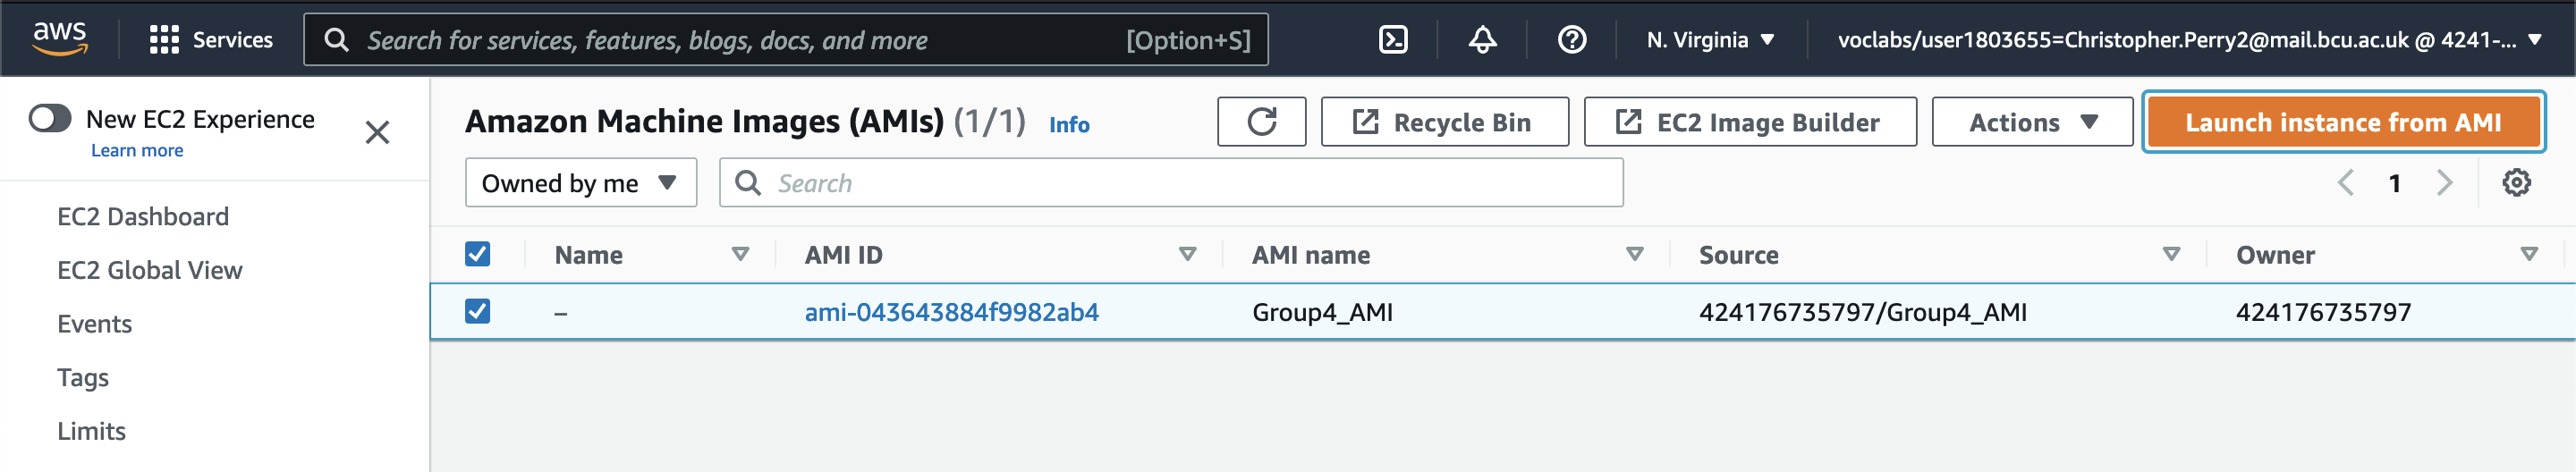
\includegraphics[width=\textwidth]{resources/elb/elb-instance-from-ami}
	  \caption{Creation of instance from AMI.}
	  \label{fig:elb-instance-from-ami}
\end{figure}

\begin{figure}[!htbp]
	  \centering
	  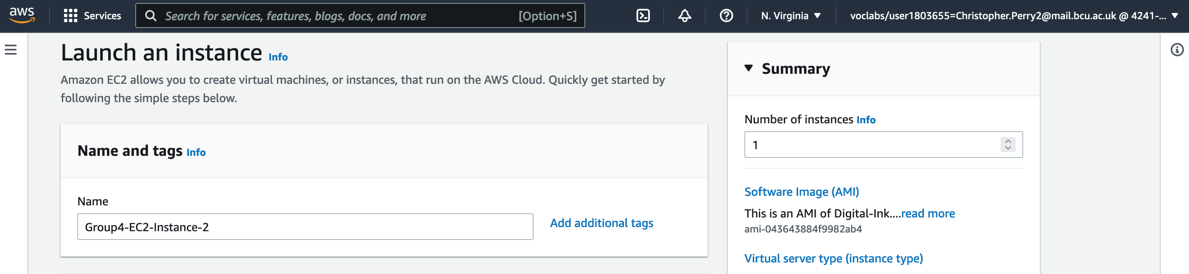
\includegraphics[width=\textwidth]{resources/elb/elb-inst-2-named}
	  \caption{Naming the second instance.}
	  \label{fig:elb-instance-2-name}
\end{figure}

\clearpage
The same KeyPair was used to make it easier to switch between the two instances.

\begin{figure}[!htbp]
	  \centering
	  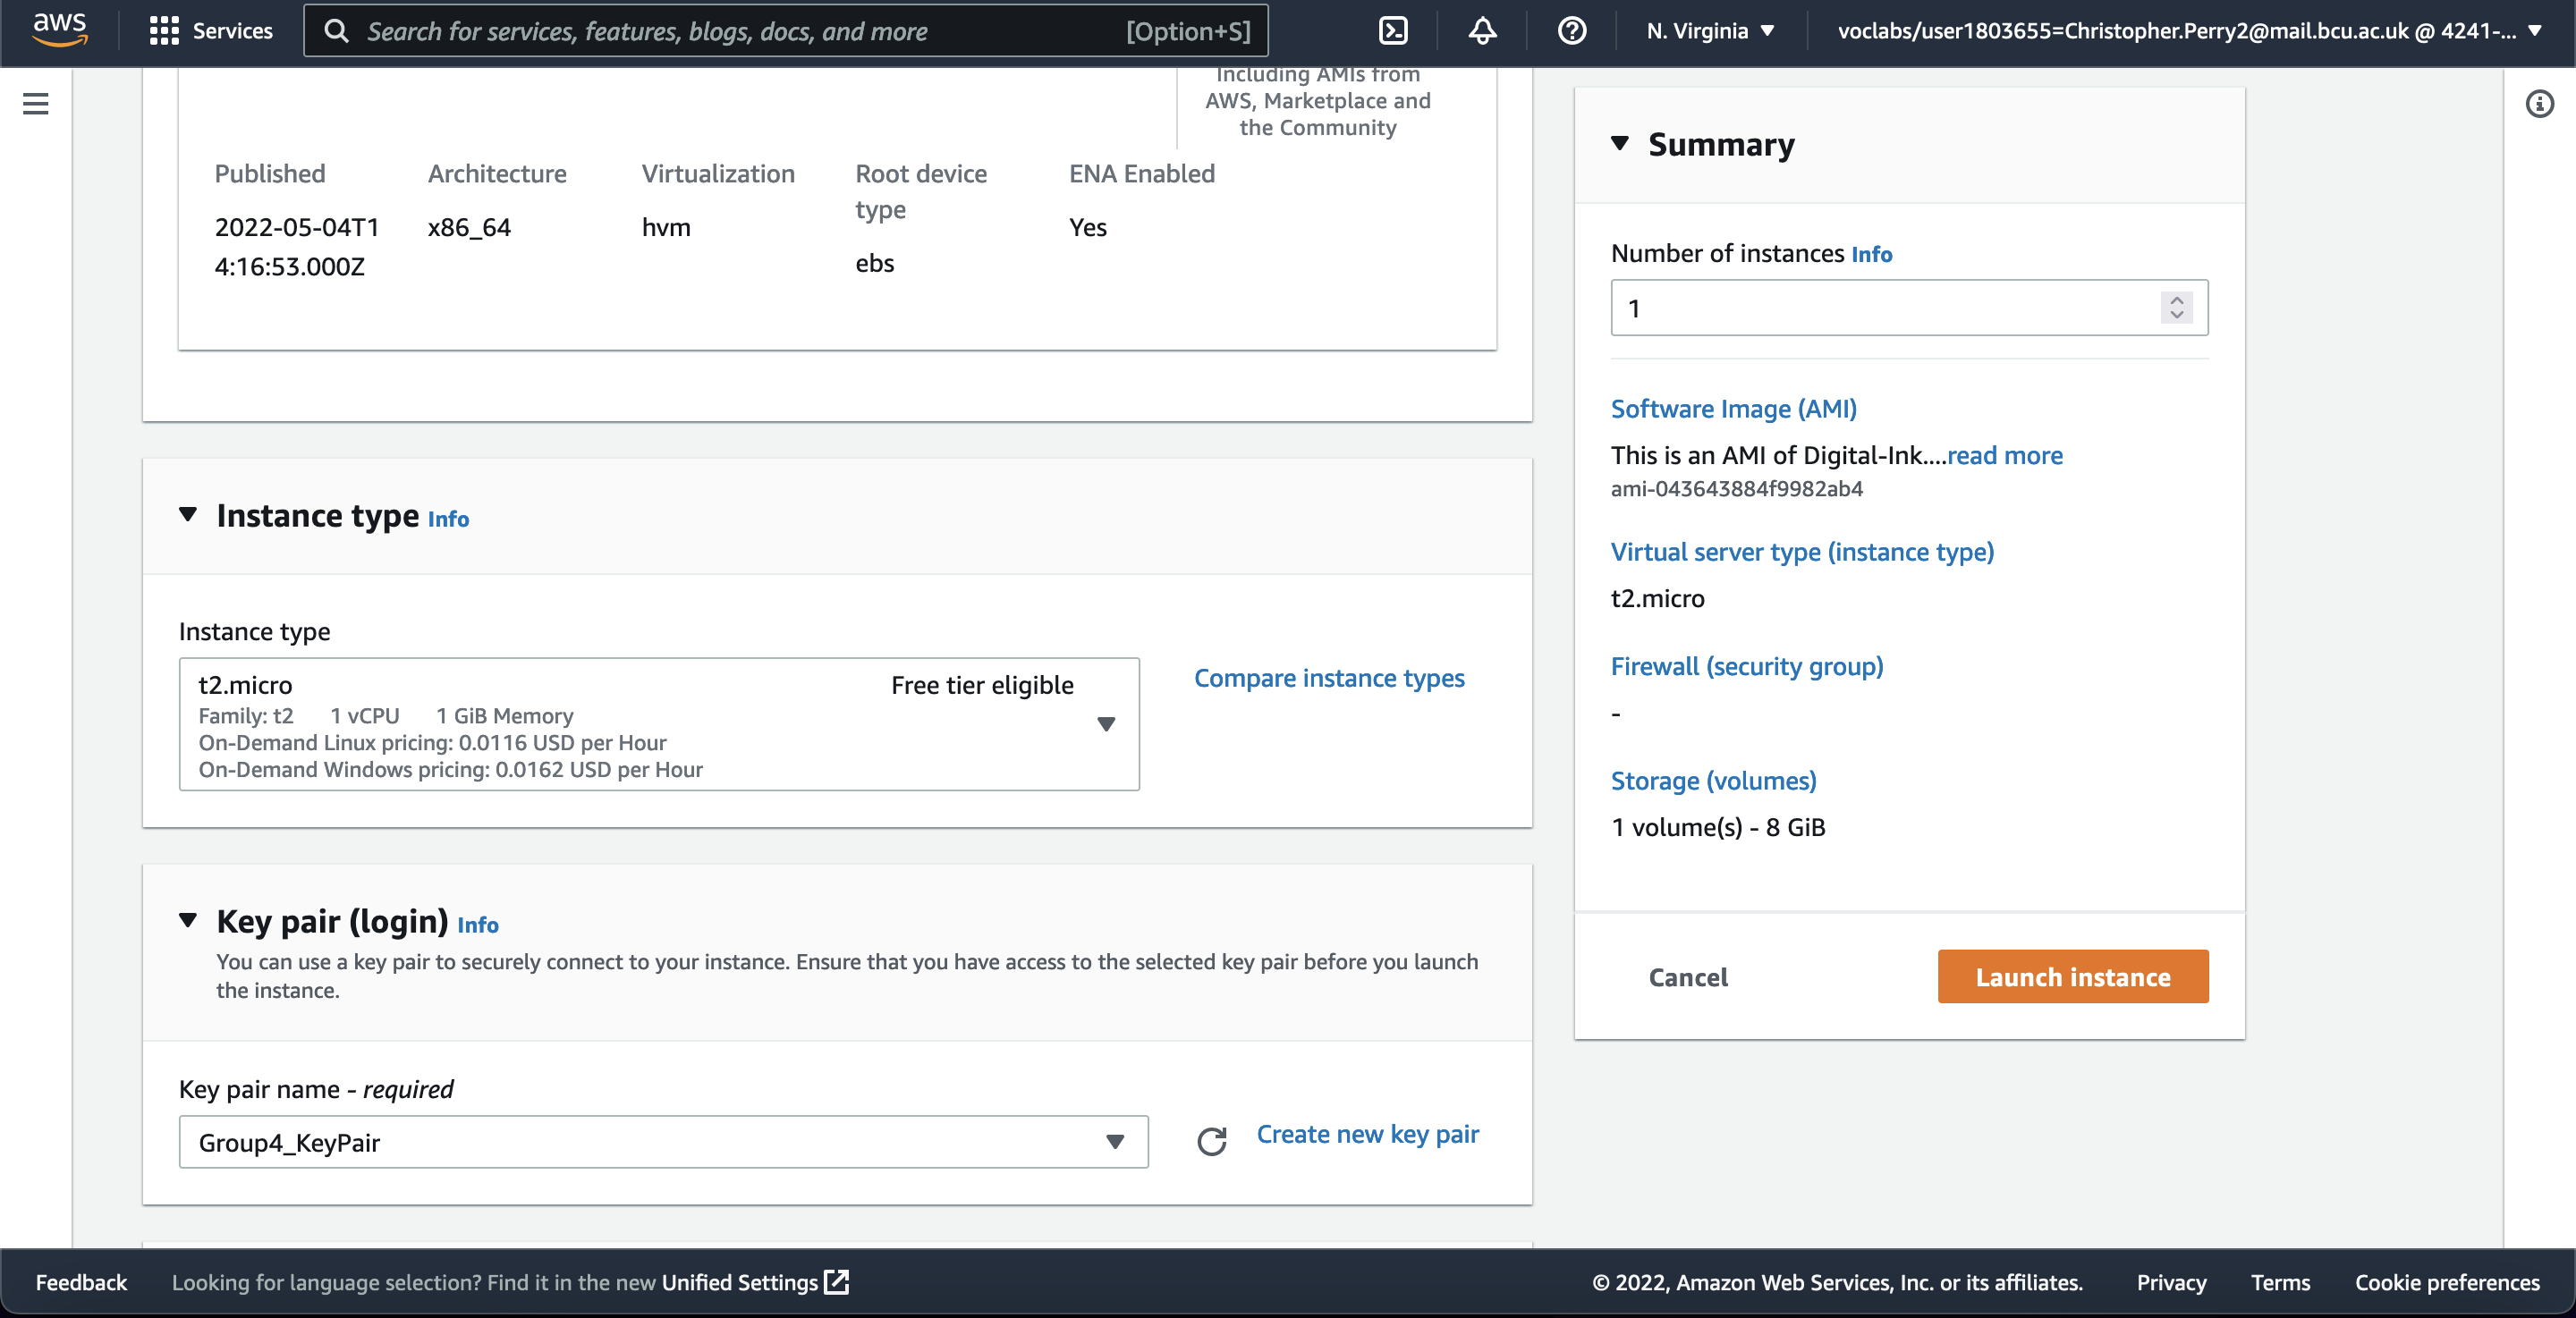
\includegraphics[width=\textwidth]{resources/elb/elb-instance-2-type-and-keypair}
	  \caption{Selection of KeyPair and instance size.}
	  \label{fig:elb-type-and-keypair}
\end{figure}

Next, the network settings of the instance were configured.
The VPC was set to be \mintinline{zsh}|Group4_VPC| (created in Section~\ref{ch:vpc}).
The subnet set to be "Public Subnet 2" and the public IP was automatically assigned.
The existing security group of "Group4-Security-Group" was selected to allow HTTP, HTTPS, SSH and MySQL traffic on the
instance.

\begin{figure}[!htbp]
	  \centering
	  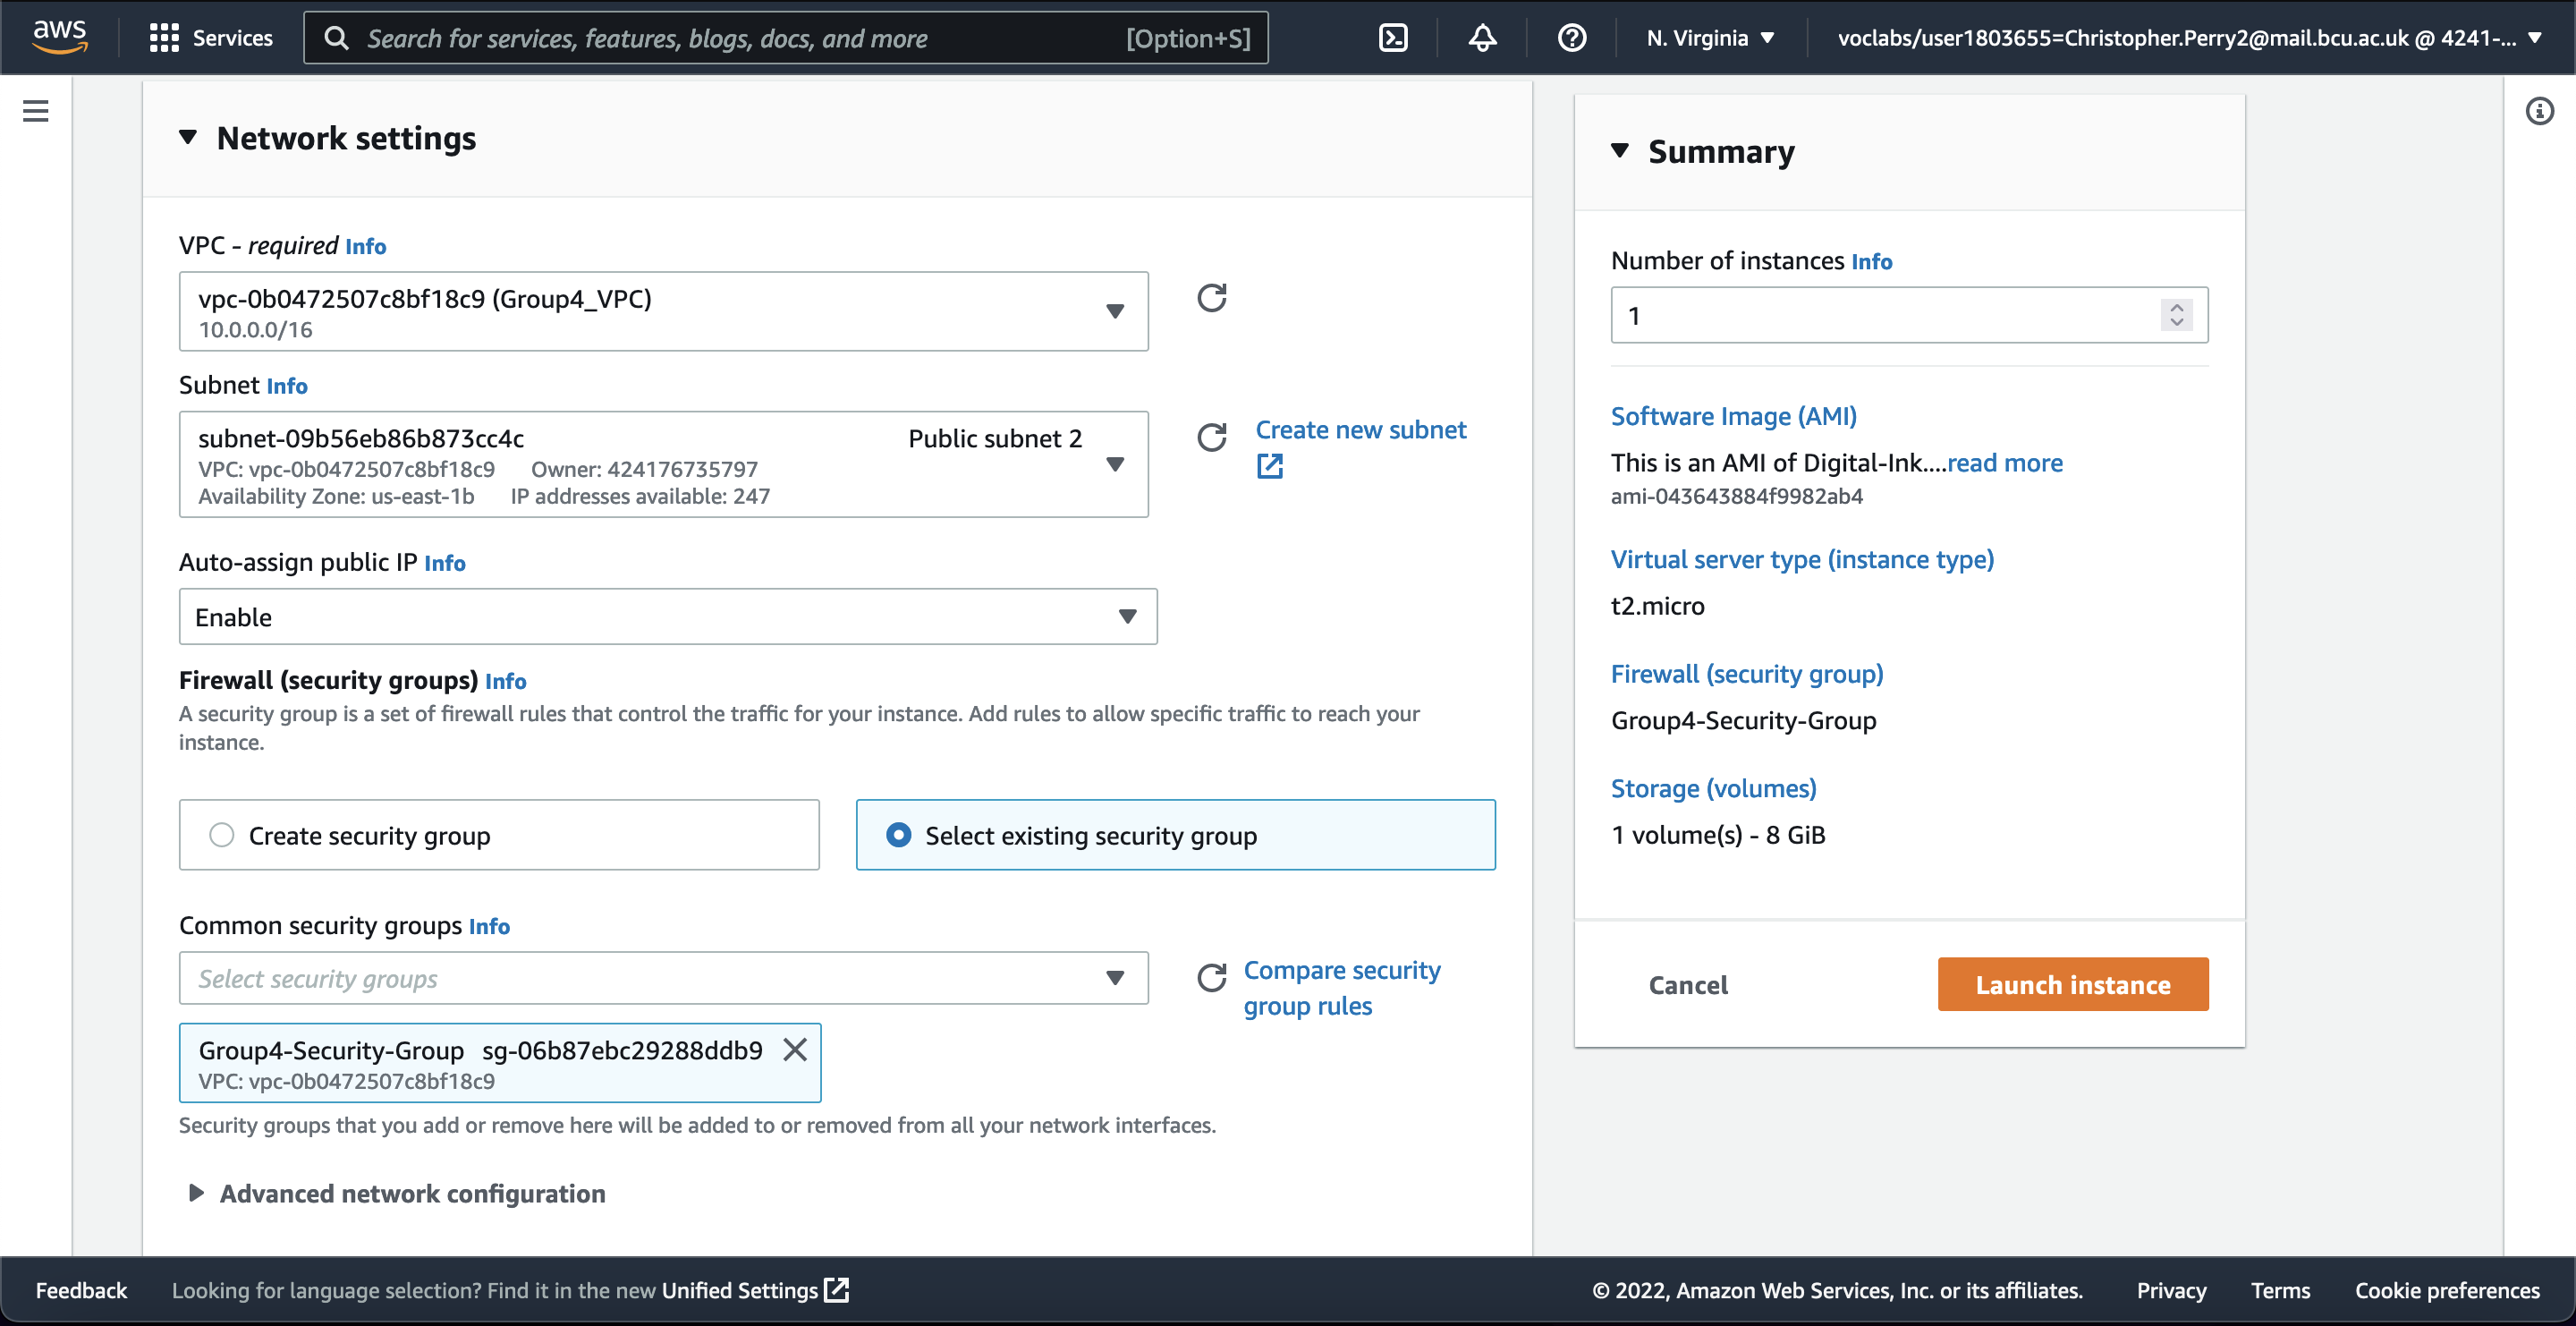
\includegraphics[width=\textwidth]{resources/elb/elb-instance-2-network-settings}
	  \caption{Selection of VPC and security group.}
	  \label{fig:elb-instance-2-network-setting}
\end{figure}

\clearpage
The storage required remained the same as previous instance.

\begin{figure}[!htbp]
	\centering
	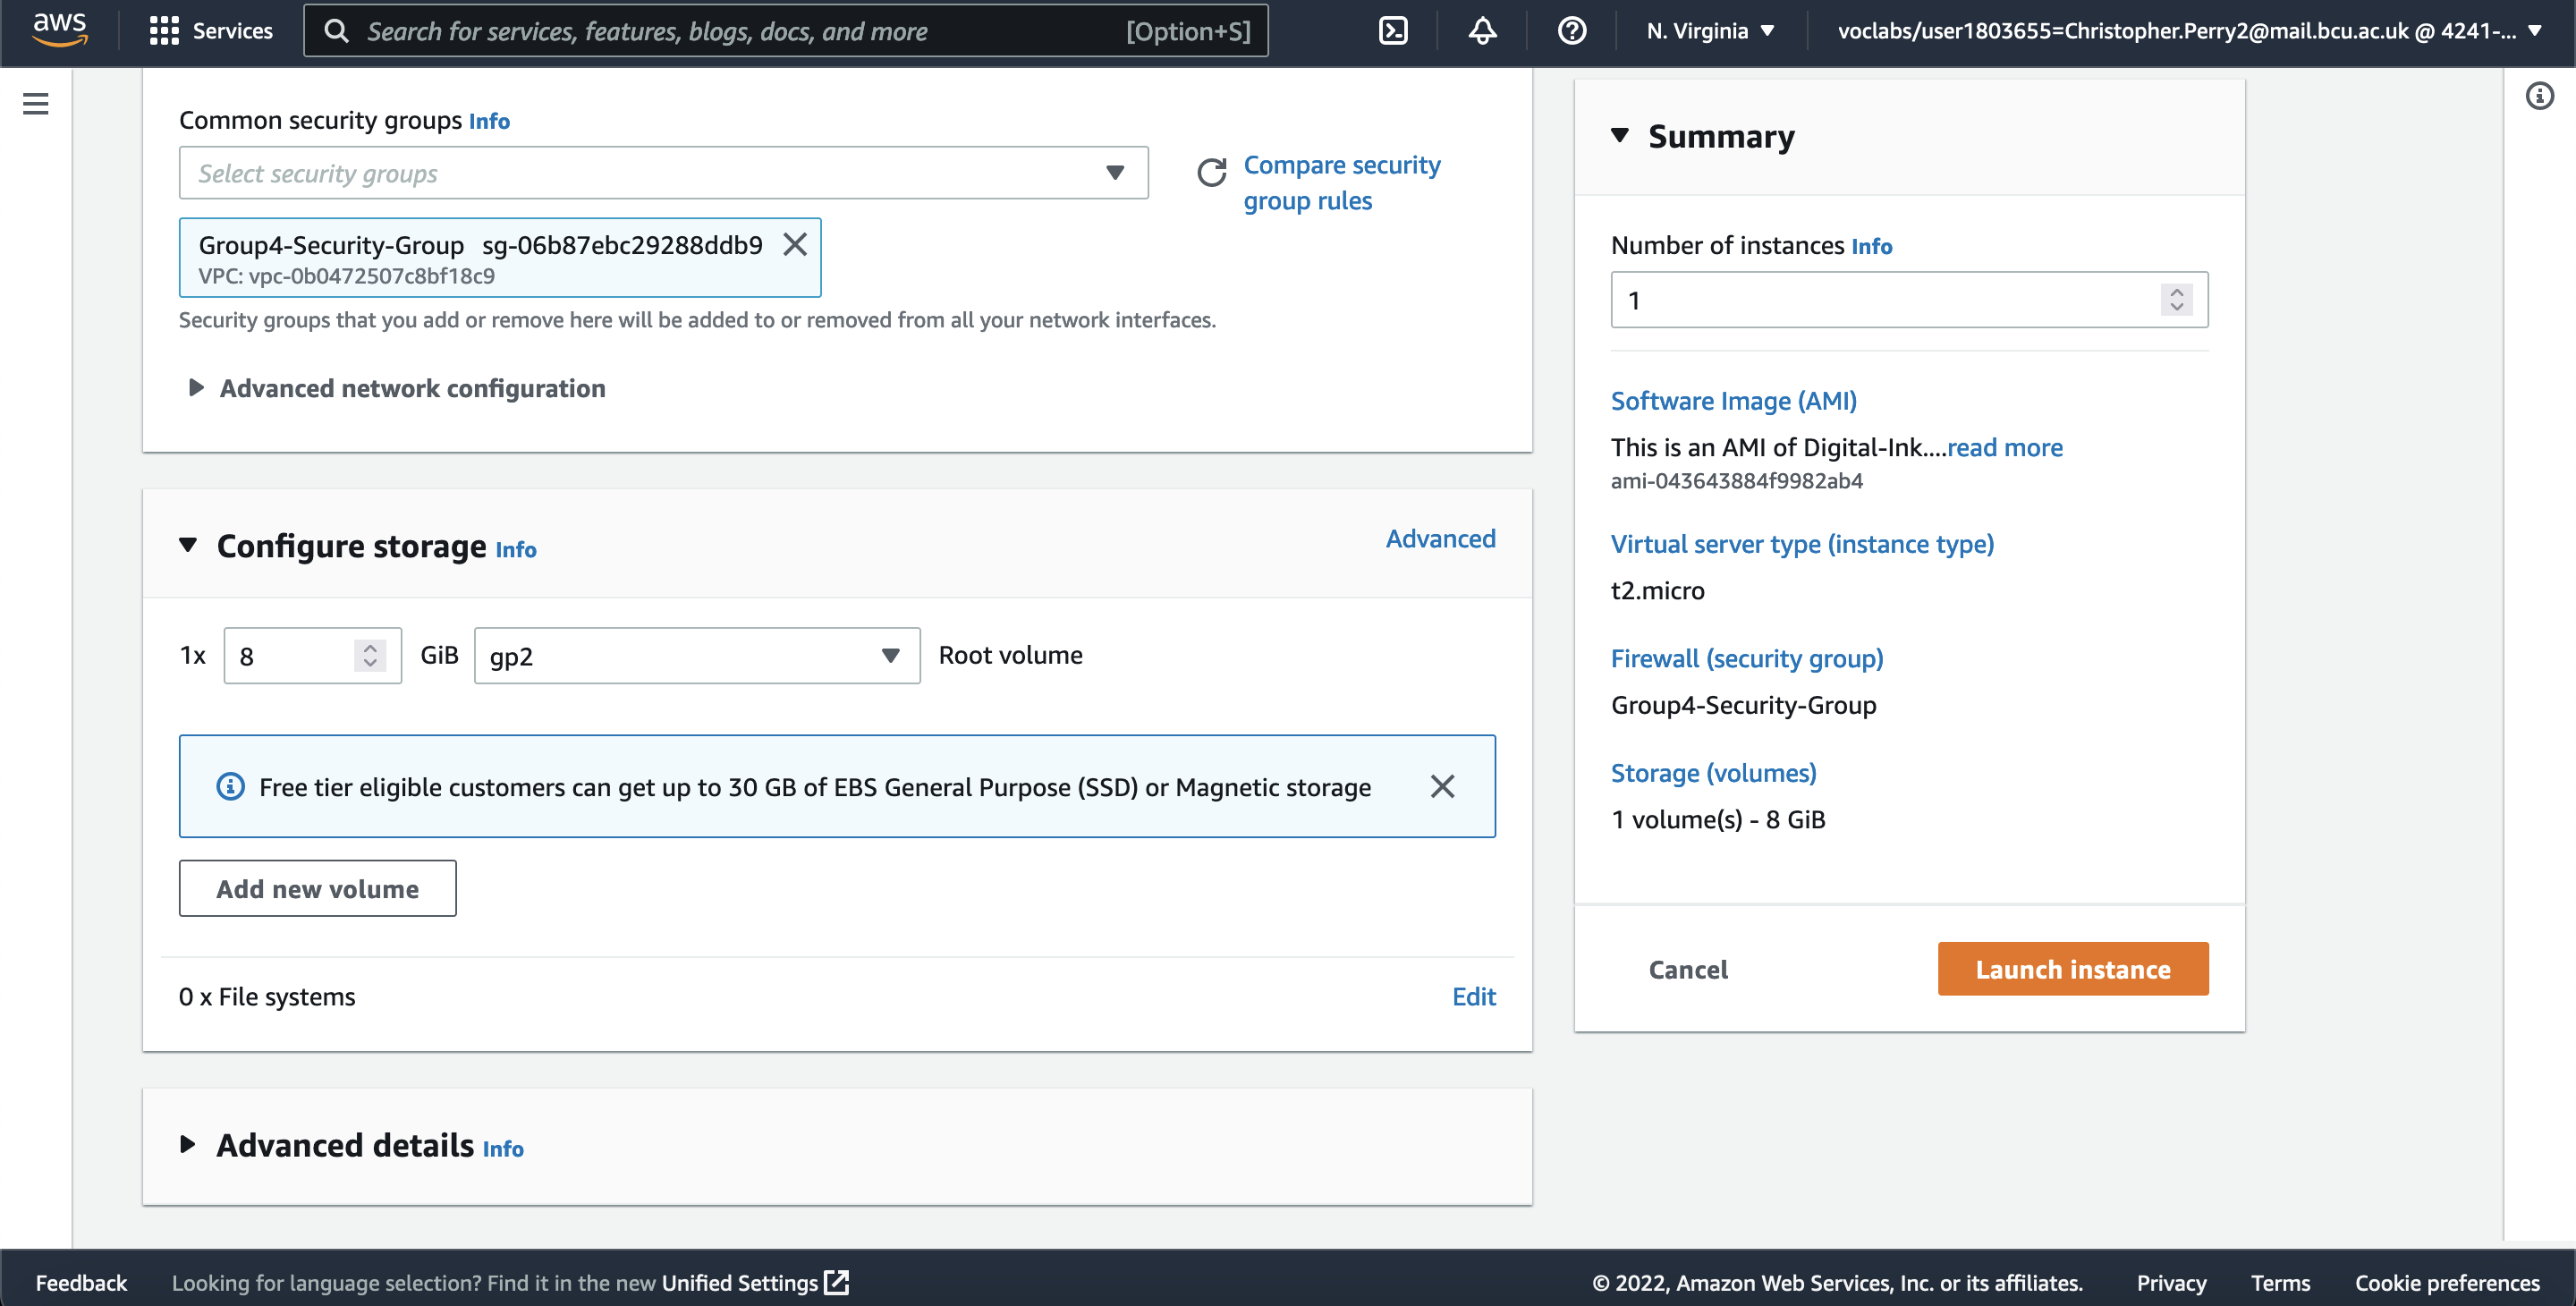
\includegraphics[width=\textwidth]{resources/elb/elb-instance-2-storage-config}
	\caption{Selection of instance storage size.}
	\label{fig:elb-instance-2-storage}
\end{figure}

After the configuration was complete, the second instance was created.
The next step is to implement an ELB to balance user load between the two instances.

\begin{figure}[!htbp]
	  \centering
	  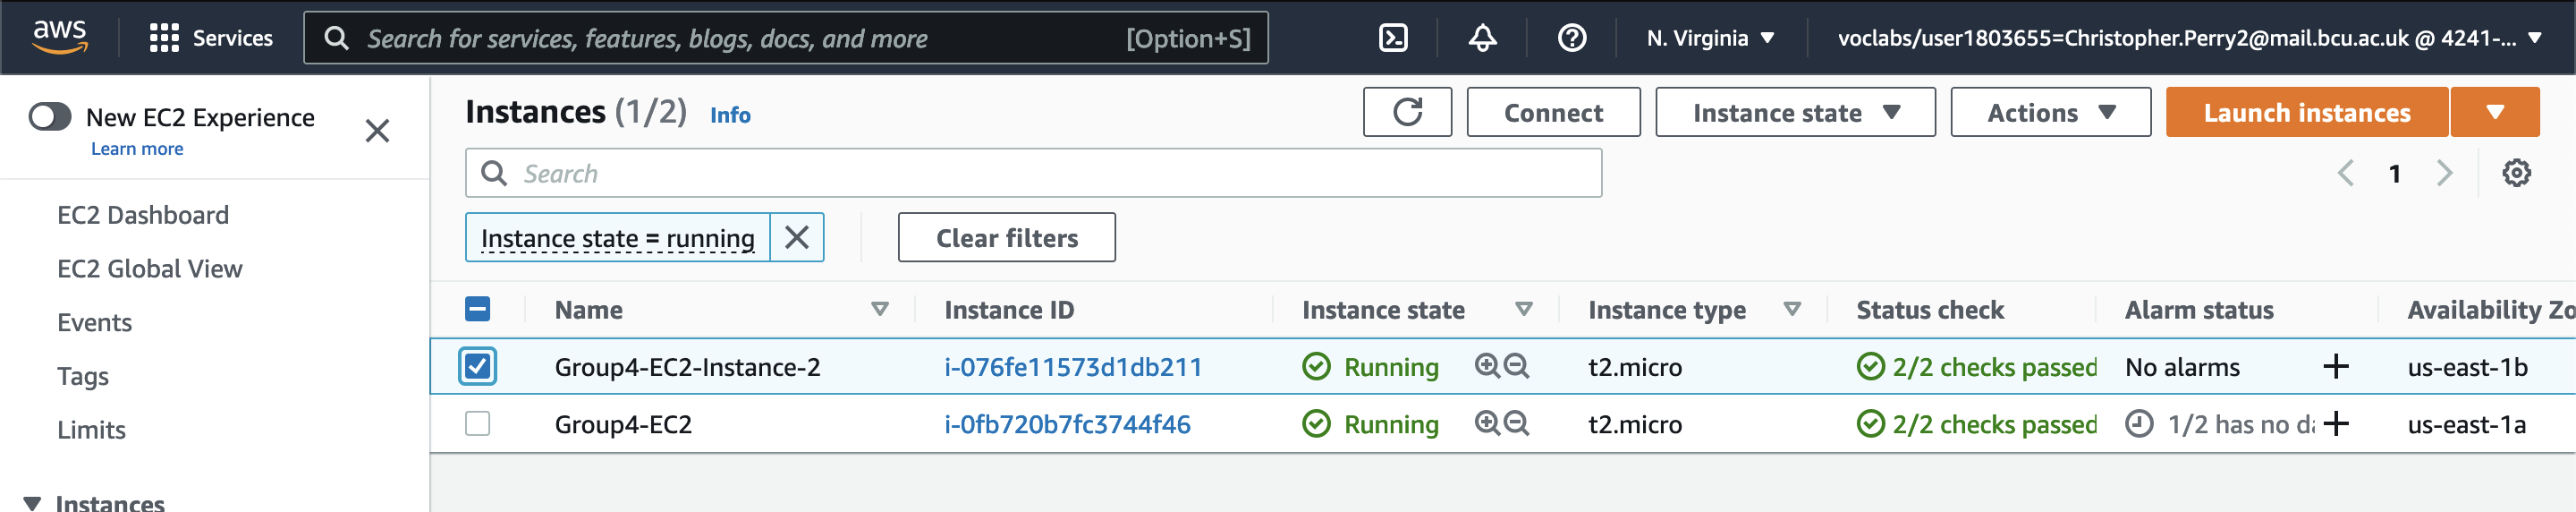
\includegraphics[width=\textwidth]{resources/elb/elb-instance-2-created}
	  \caption{Second instance creation success.}
	  \label{fig:elb-instance-2-create}
\end{figure}

\clearpage
\section{Creating a Target Group}\label{sec:creating-a-target-group}

Now that there are two instances, they both need to be stored within a target group.
The target group type of "Instances" was selected - this will store both running instances of \textit{Digital-Ink} in a
target group to be handled by the ELB\@.
The target group was assigned a name of "Group4-Target-Group" and given a protocol of HTTP and port 80.

\begin{figure}[!htbp]
	 \centering
	 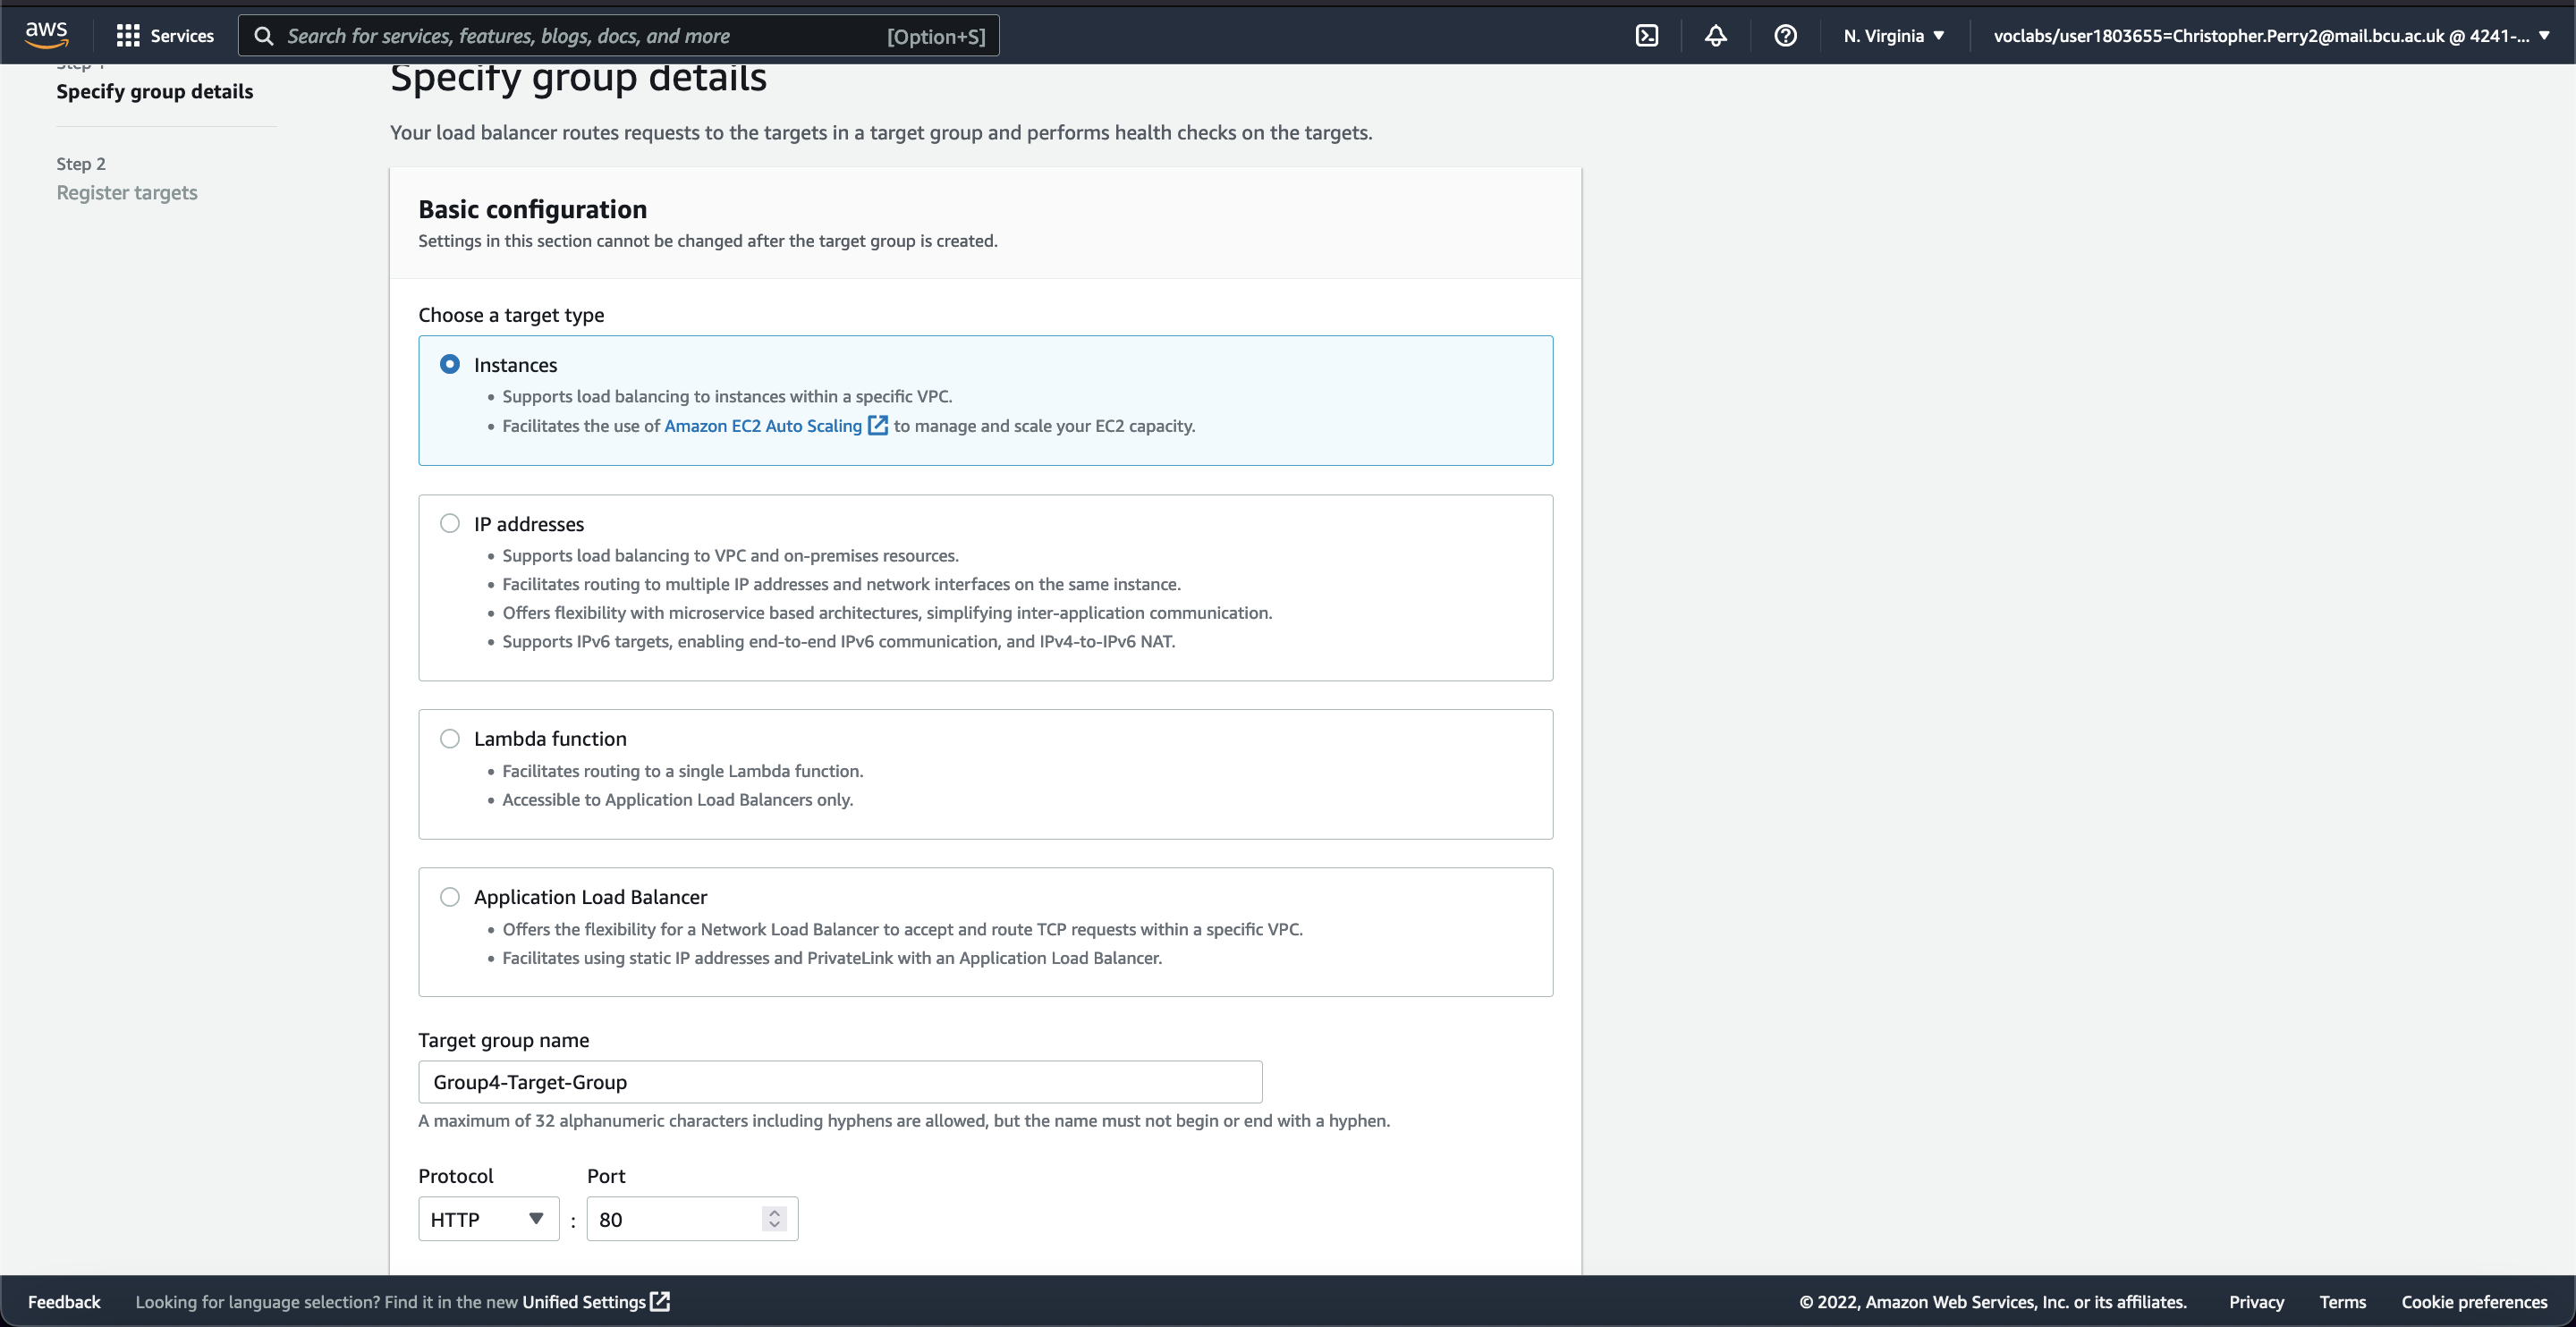
\includegraphics[width=\textwidth]{resources/elb/elb-target-group-basic-config}
	 \caption{Setting target type, protocol and port.}
	 \label{fig:elb-target-group-basic-config}
\end{figure}

\begin{figure}[!htbp]
	  \centering
	  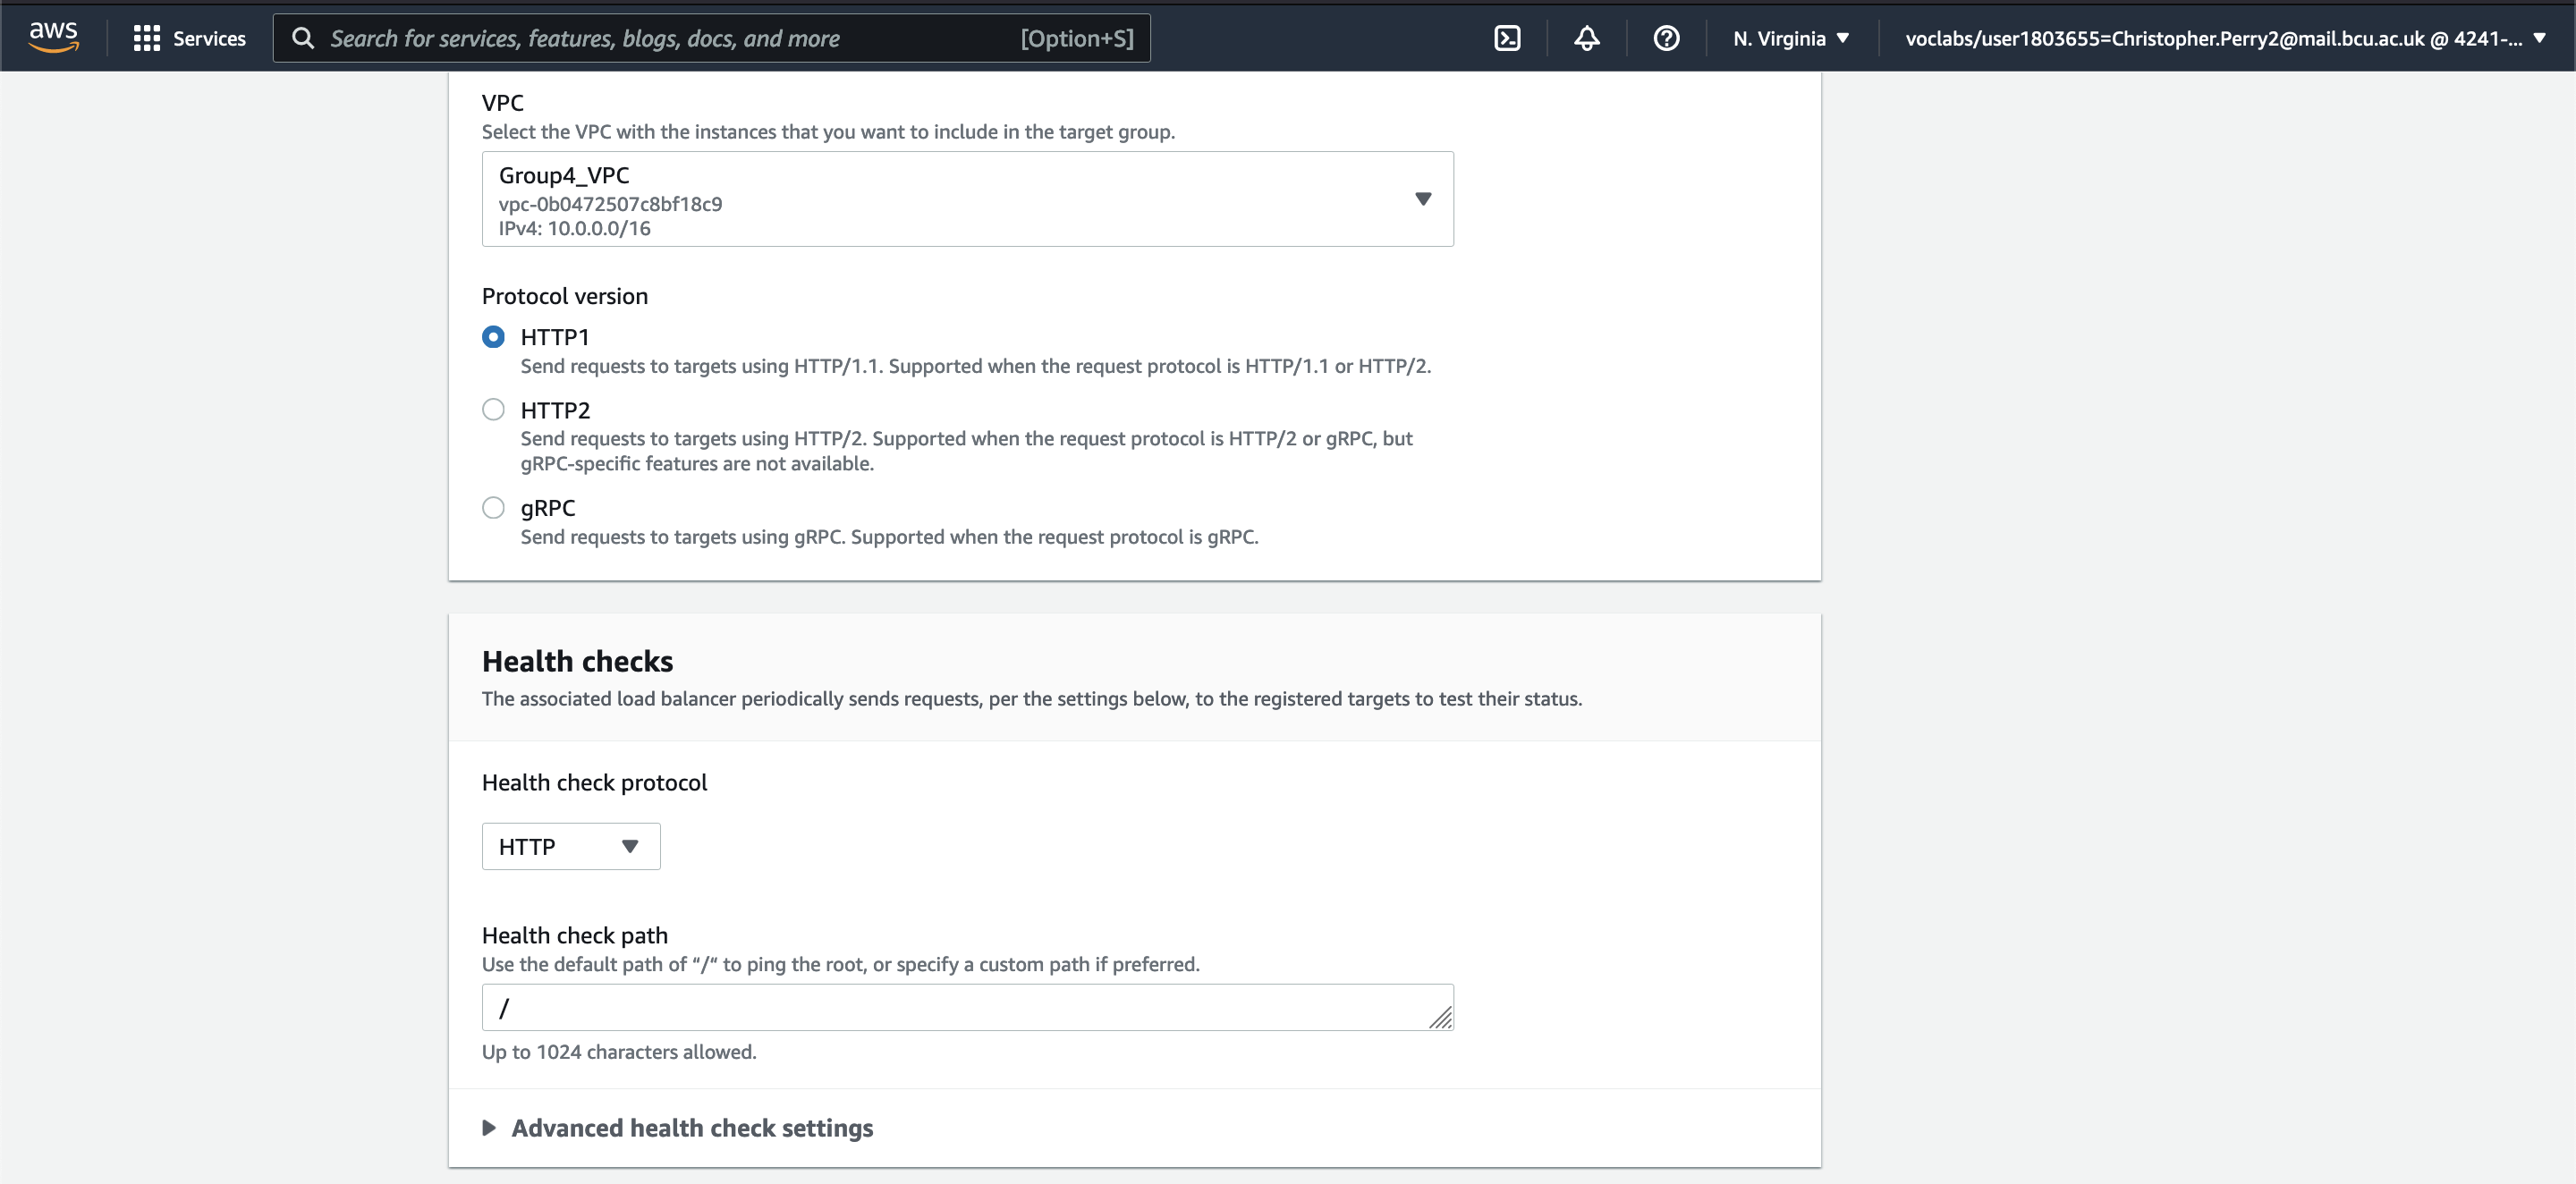
\includegraphics[width=\textwidth]{resources/elb/elb-vpc}
	  \caption{Selection of group 4 VPC.}
	  \label{fig:elb-vpc}
\end{figure}

\clearpage
The next screen asks for instances that will be registered to the target group to be selected.
The two running instances of \textit{Digital-Ink} are shown and added as targets through the
\textbf{Include as pending below} button.

\begin{figure}[!htbp]
	  \centering
	  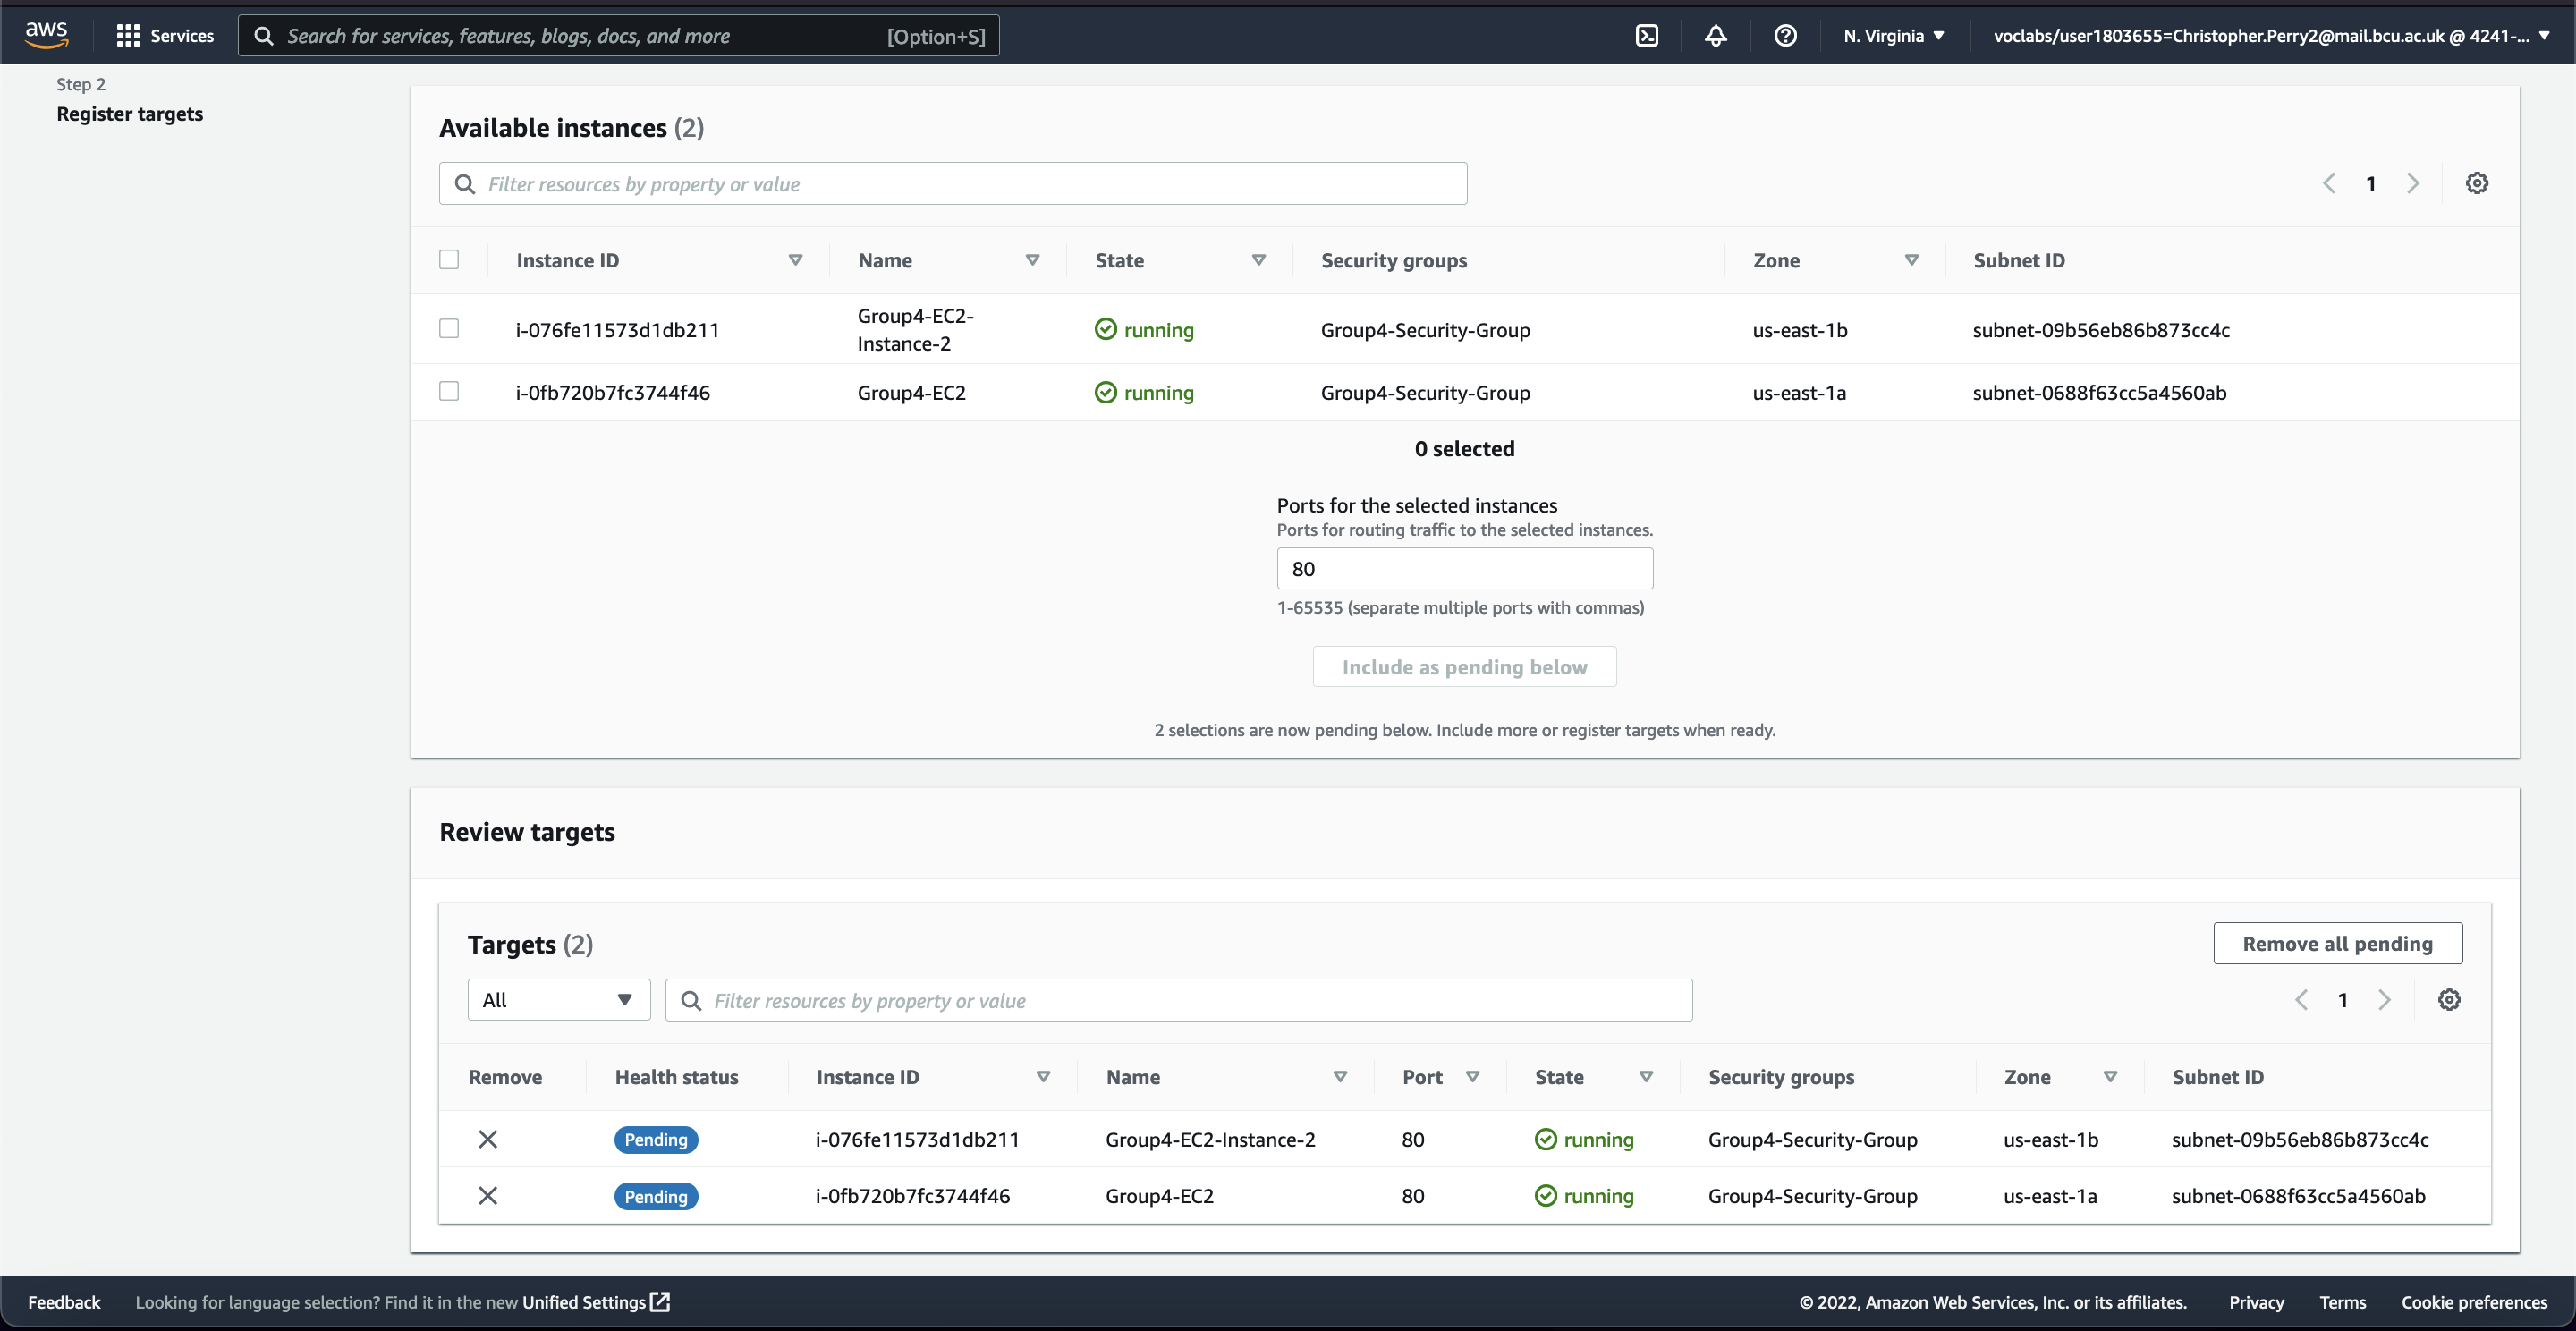
\includegraphics[width=\textwidth]{resources/elb/elb-register-targets}
	  \caption{Include as pending below.}
	  \label{fig:elb-register-targets}
\end{figure}

The target group has now been created and contains both EC2 instances.

\begin{figure}[!htbp]
	  \centering
	  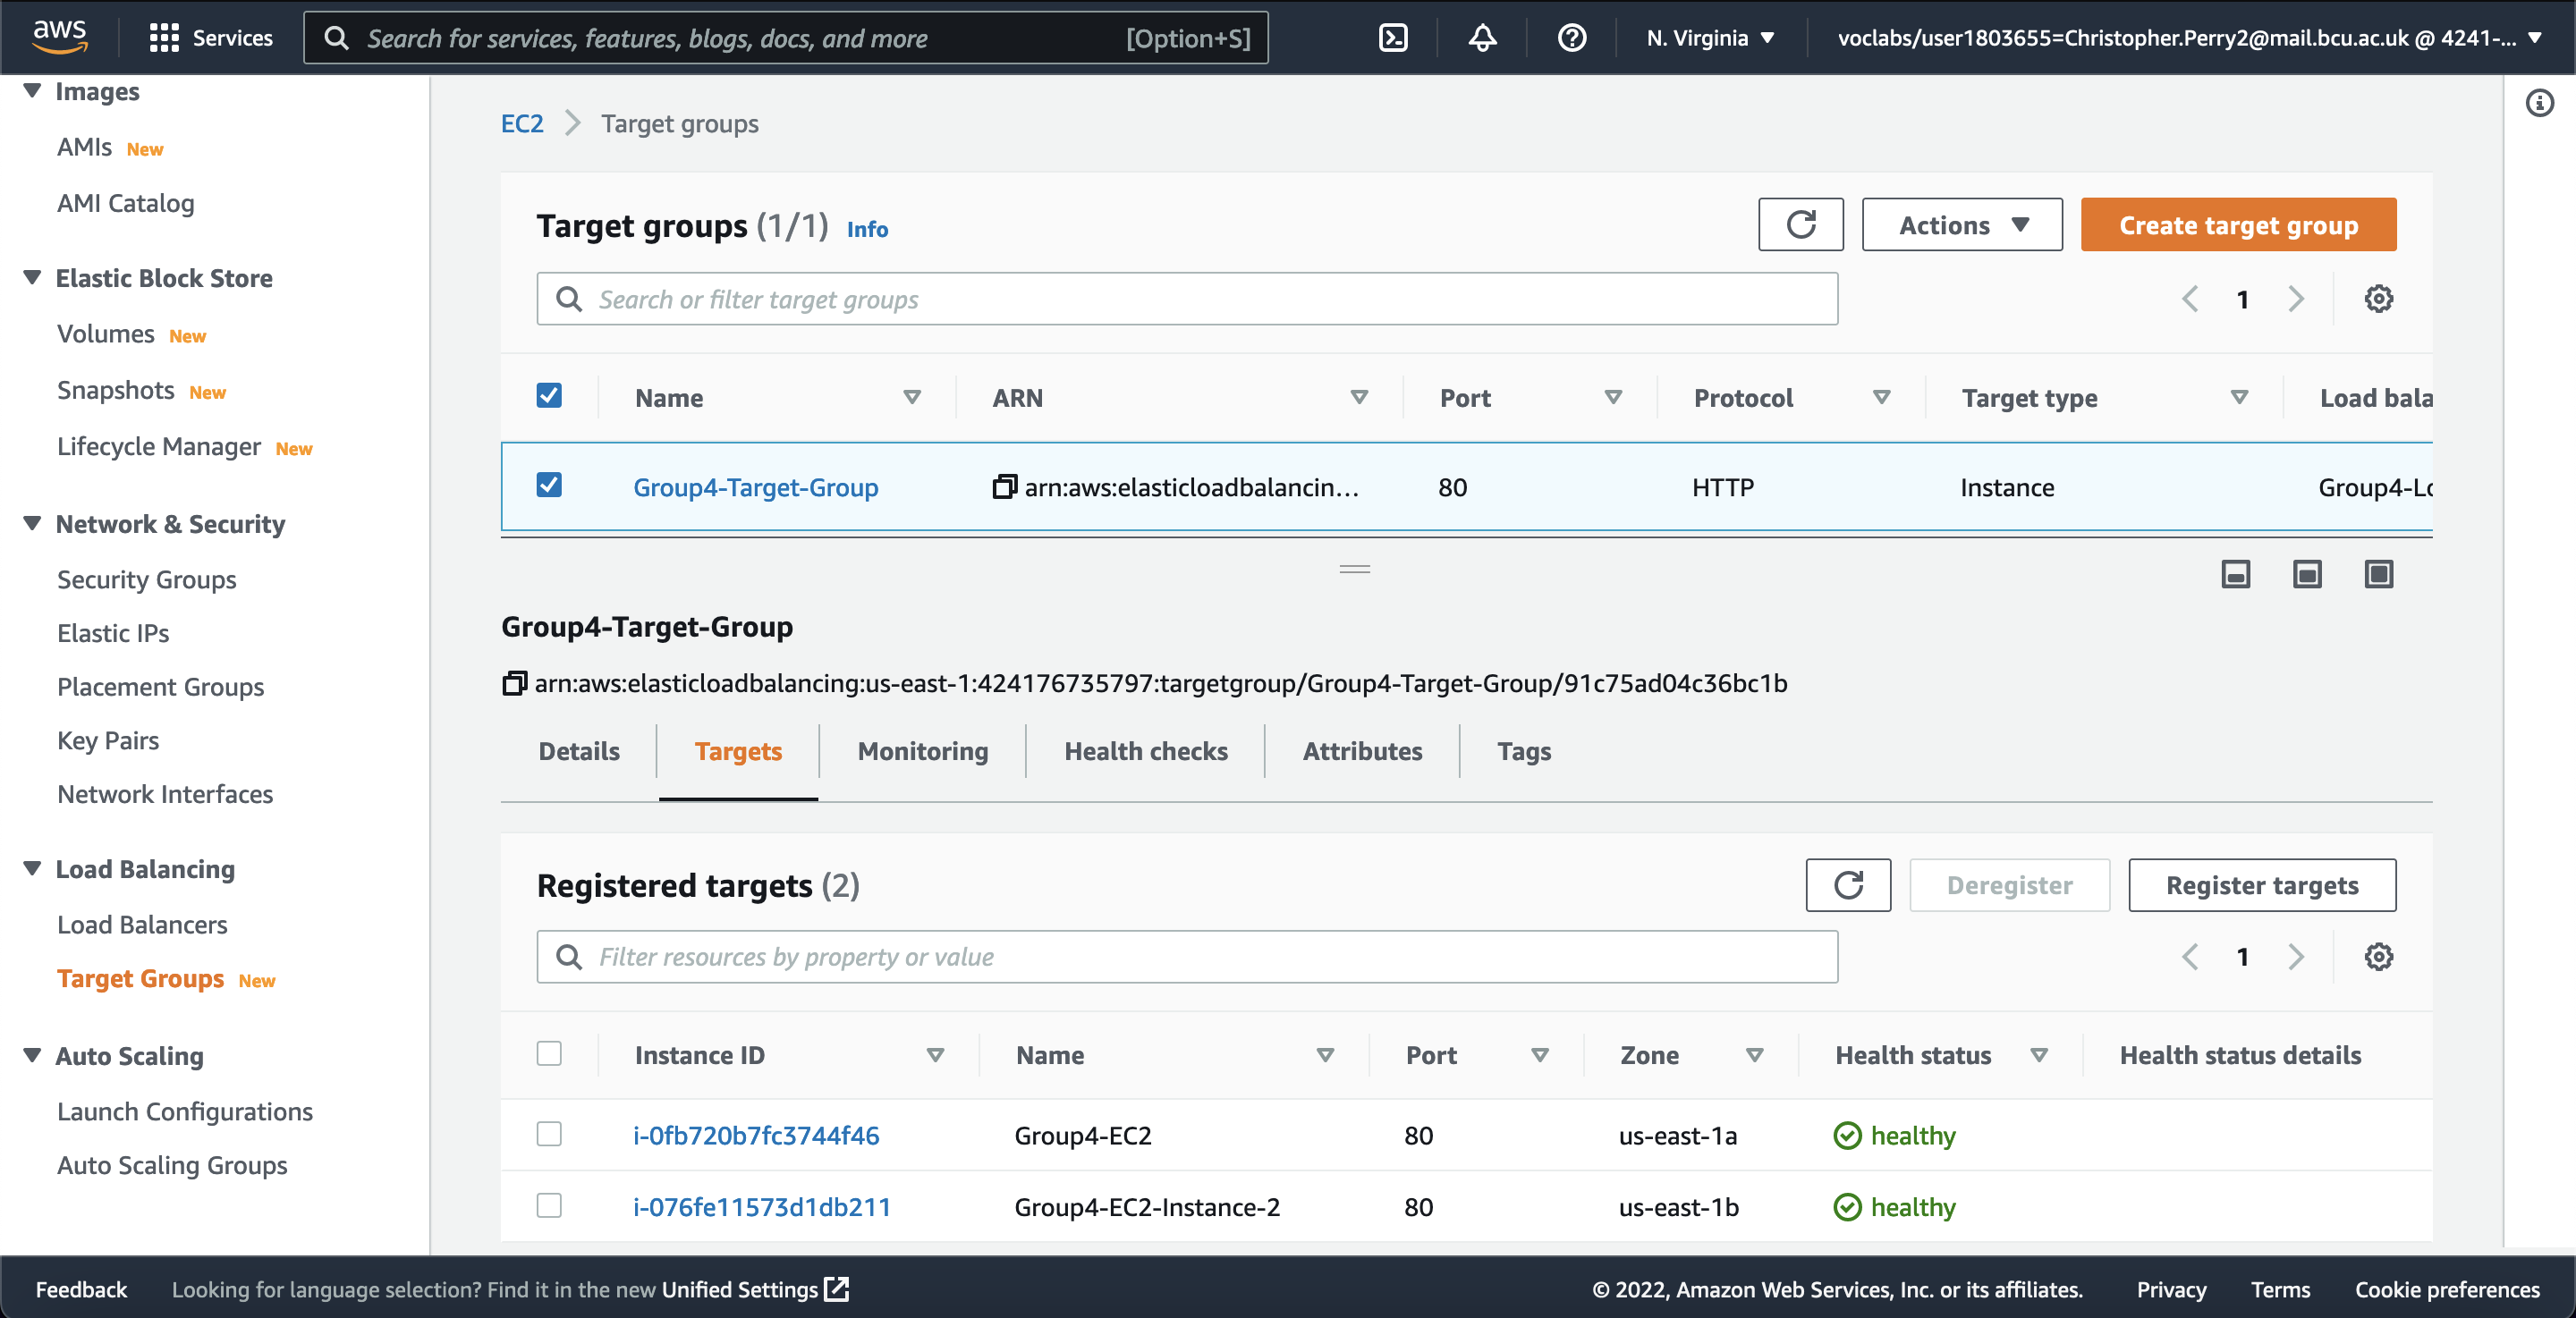
\includegraphics[width=\textwidth]{resources/elb/elb-target-group-created}
	  \caption{Target groups success.}
	  \label{fig:elb-target-group-create}
\end{figure}

\clearpage
\section{Creating a Load Balancer}\label{sec:creating-a-load-balancer}

The Target groups are not associated with a Load Balancer, so one will be created as an Application Load Balancer with
the name "Group4-Load-Balancer".

\begin{figure}[!htbp]
	\centering
	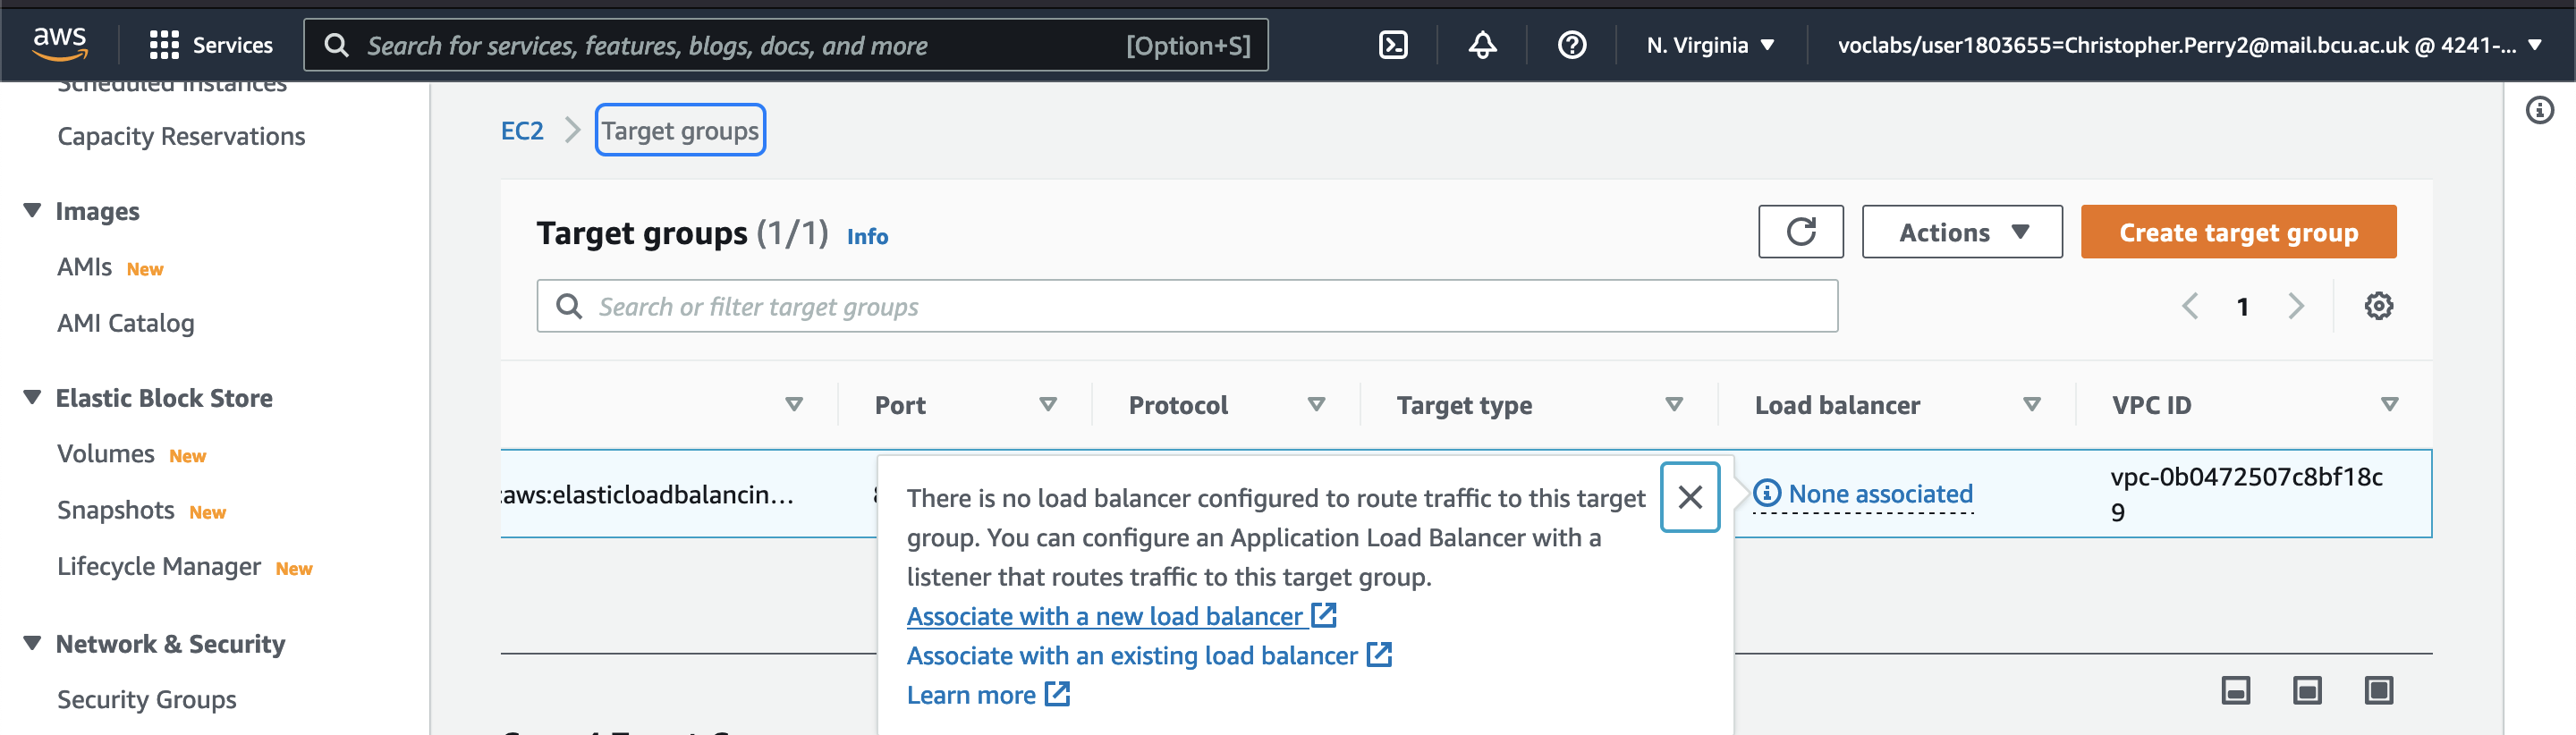
\includegraphics[width=120mm]{resources/elb/elb-load-balancer-creation}
	\caption{No load balancer configured warning.}
	\label{fig:elb-load-bal-create}
\end{figure}

\begin{figure}[!htbp]
	\centering
	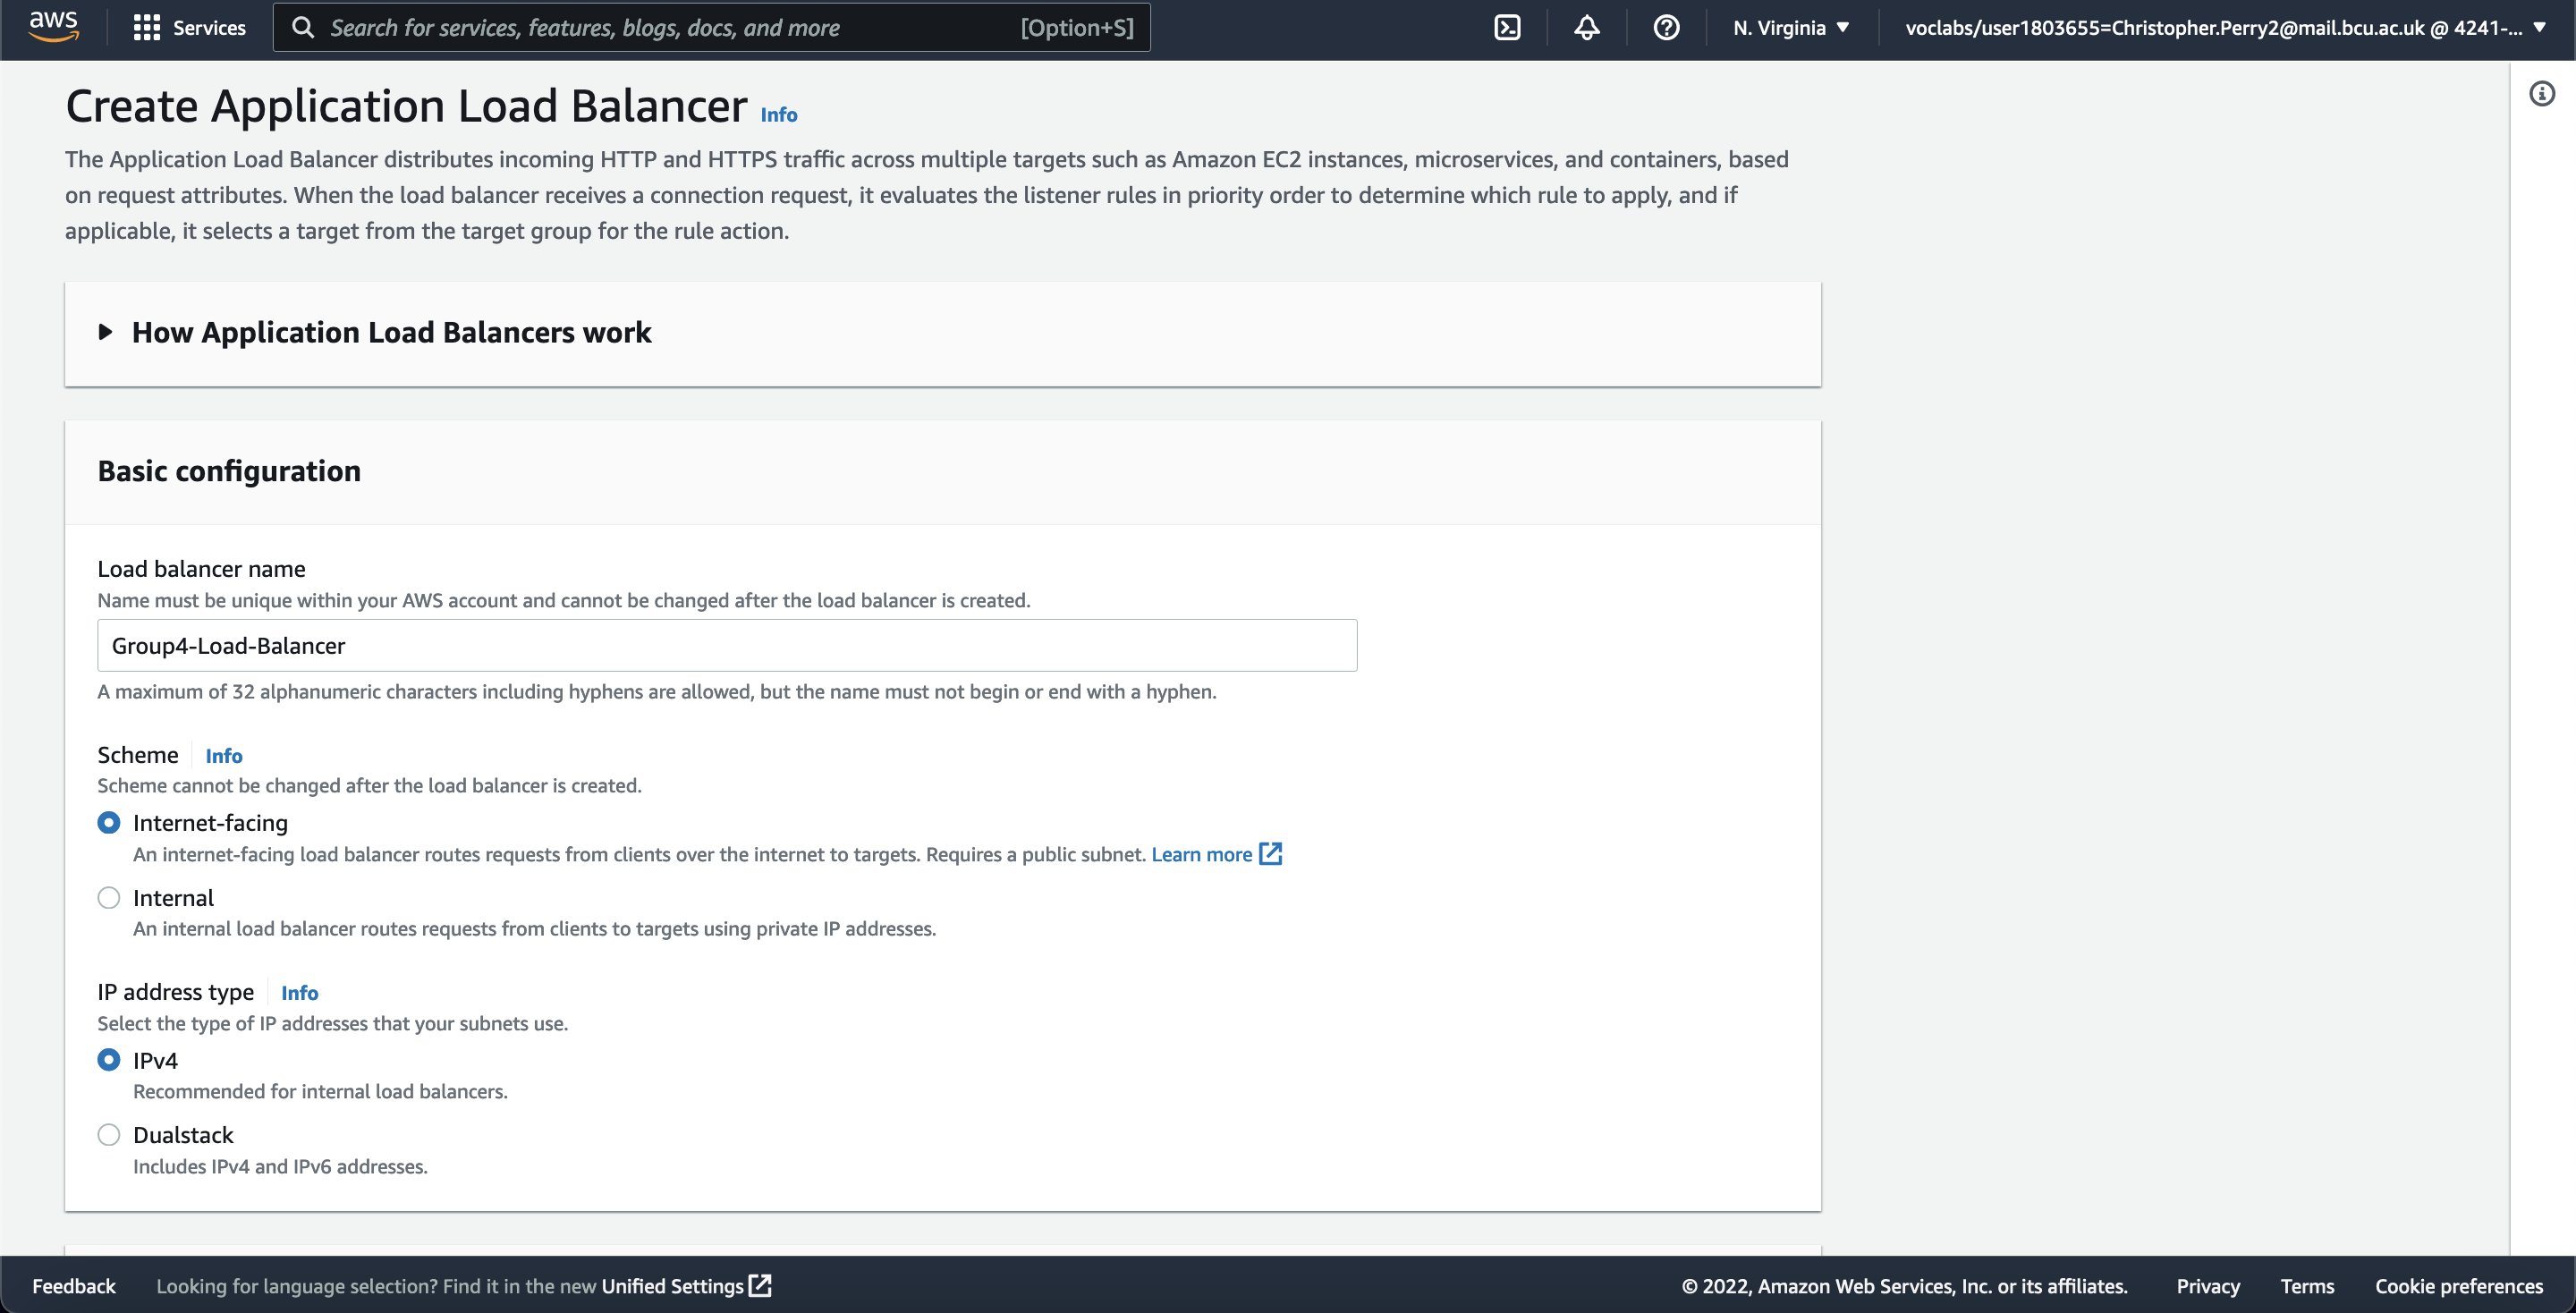
\includegraphics[width=120mm]{resources/elb/elb-basic-config}
	\caption{Load balancer creation.}
	\label{fig:elb-creation-config}
\end{figure}

The Load Balancer was additionally set to be internet facing and to handle IPv4 addresses.

\begin{figure}[!htbp]
	\centering
	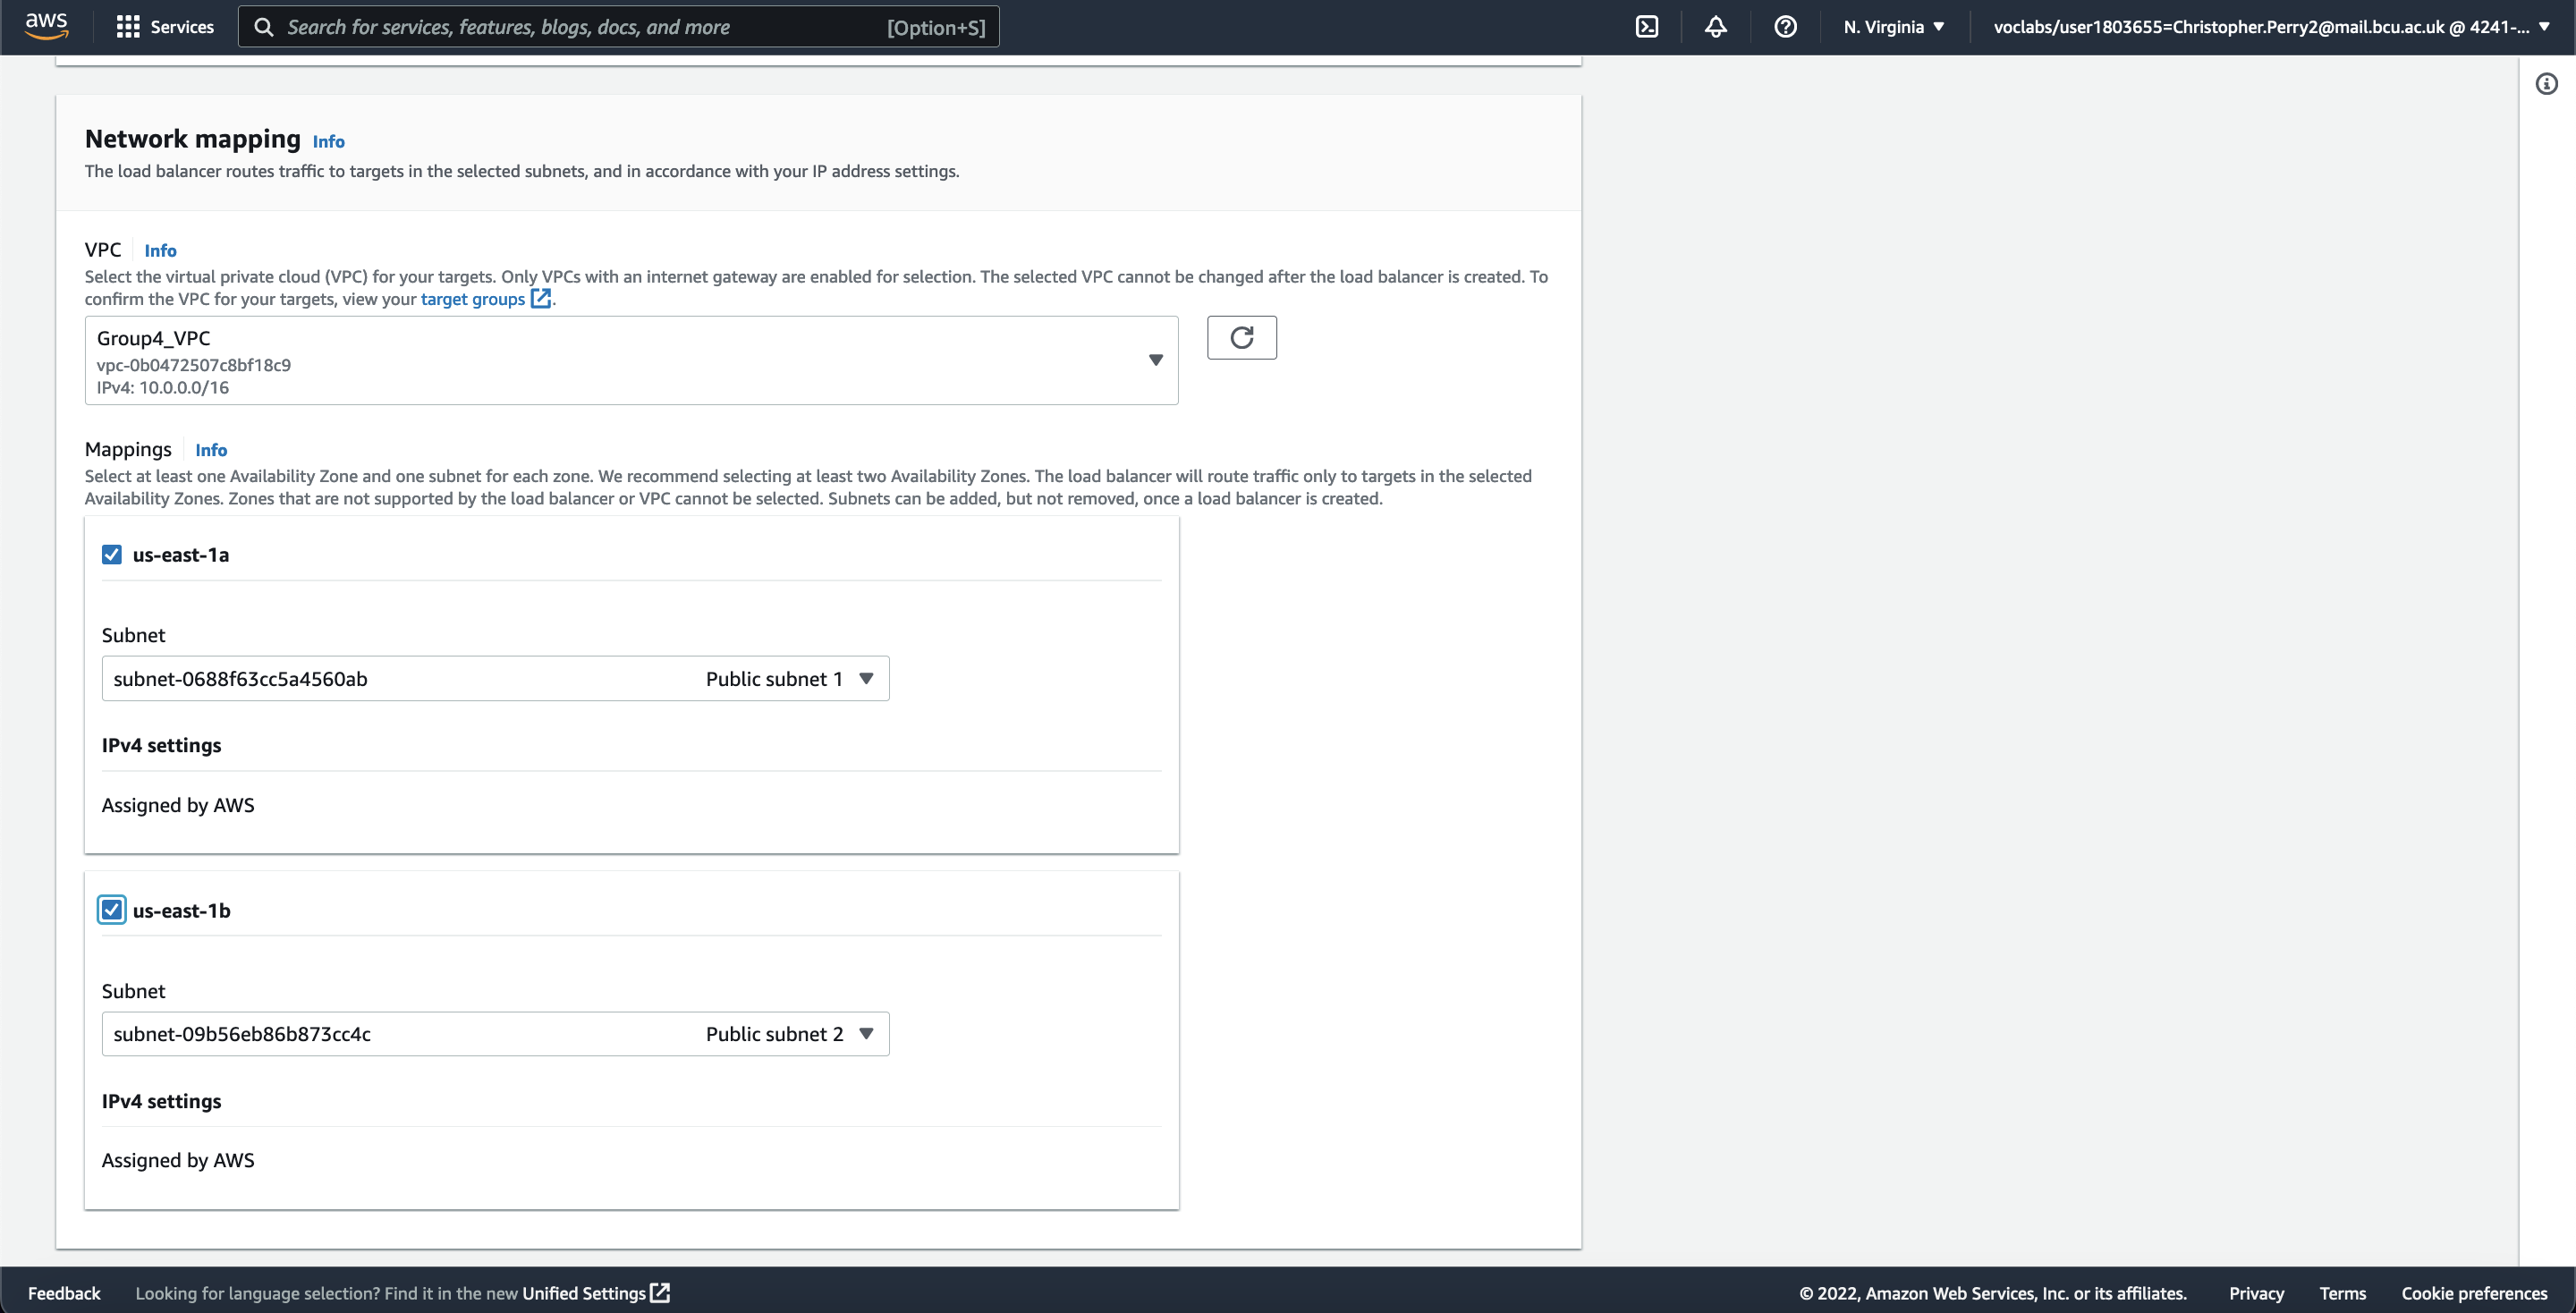
\includegraphics[width=120mm]{resources/elb/elb-network-mapping}
	\caption{Load balancer network mapping.}
	\label{fig:elb-network-mapping}
\end{figure}

\clearpage
The security group of "Group4-Security-Group" was selected, which allows HTTP, HTTPS, SSH and MySQL traffic within
the load balancer.
In the event that either of the web app instances become unavailable, it will be forwarded to the Group4-Target-Group,
which will then display the available instance.

\begin{figure}[!htbp]
	\centering
	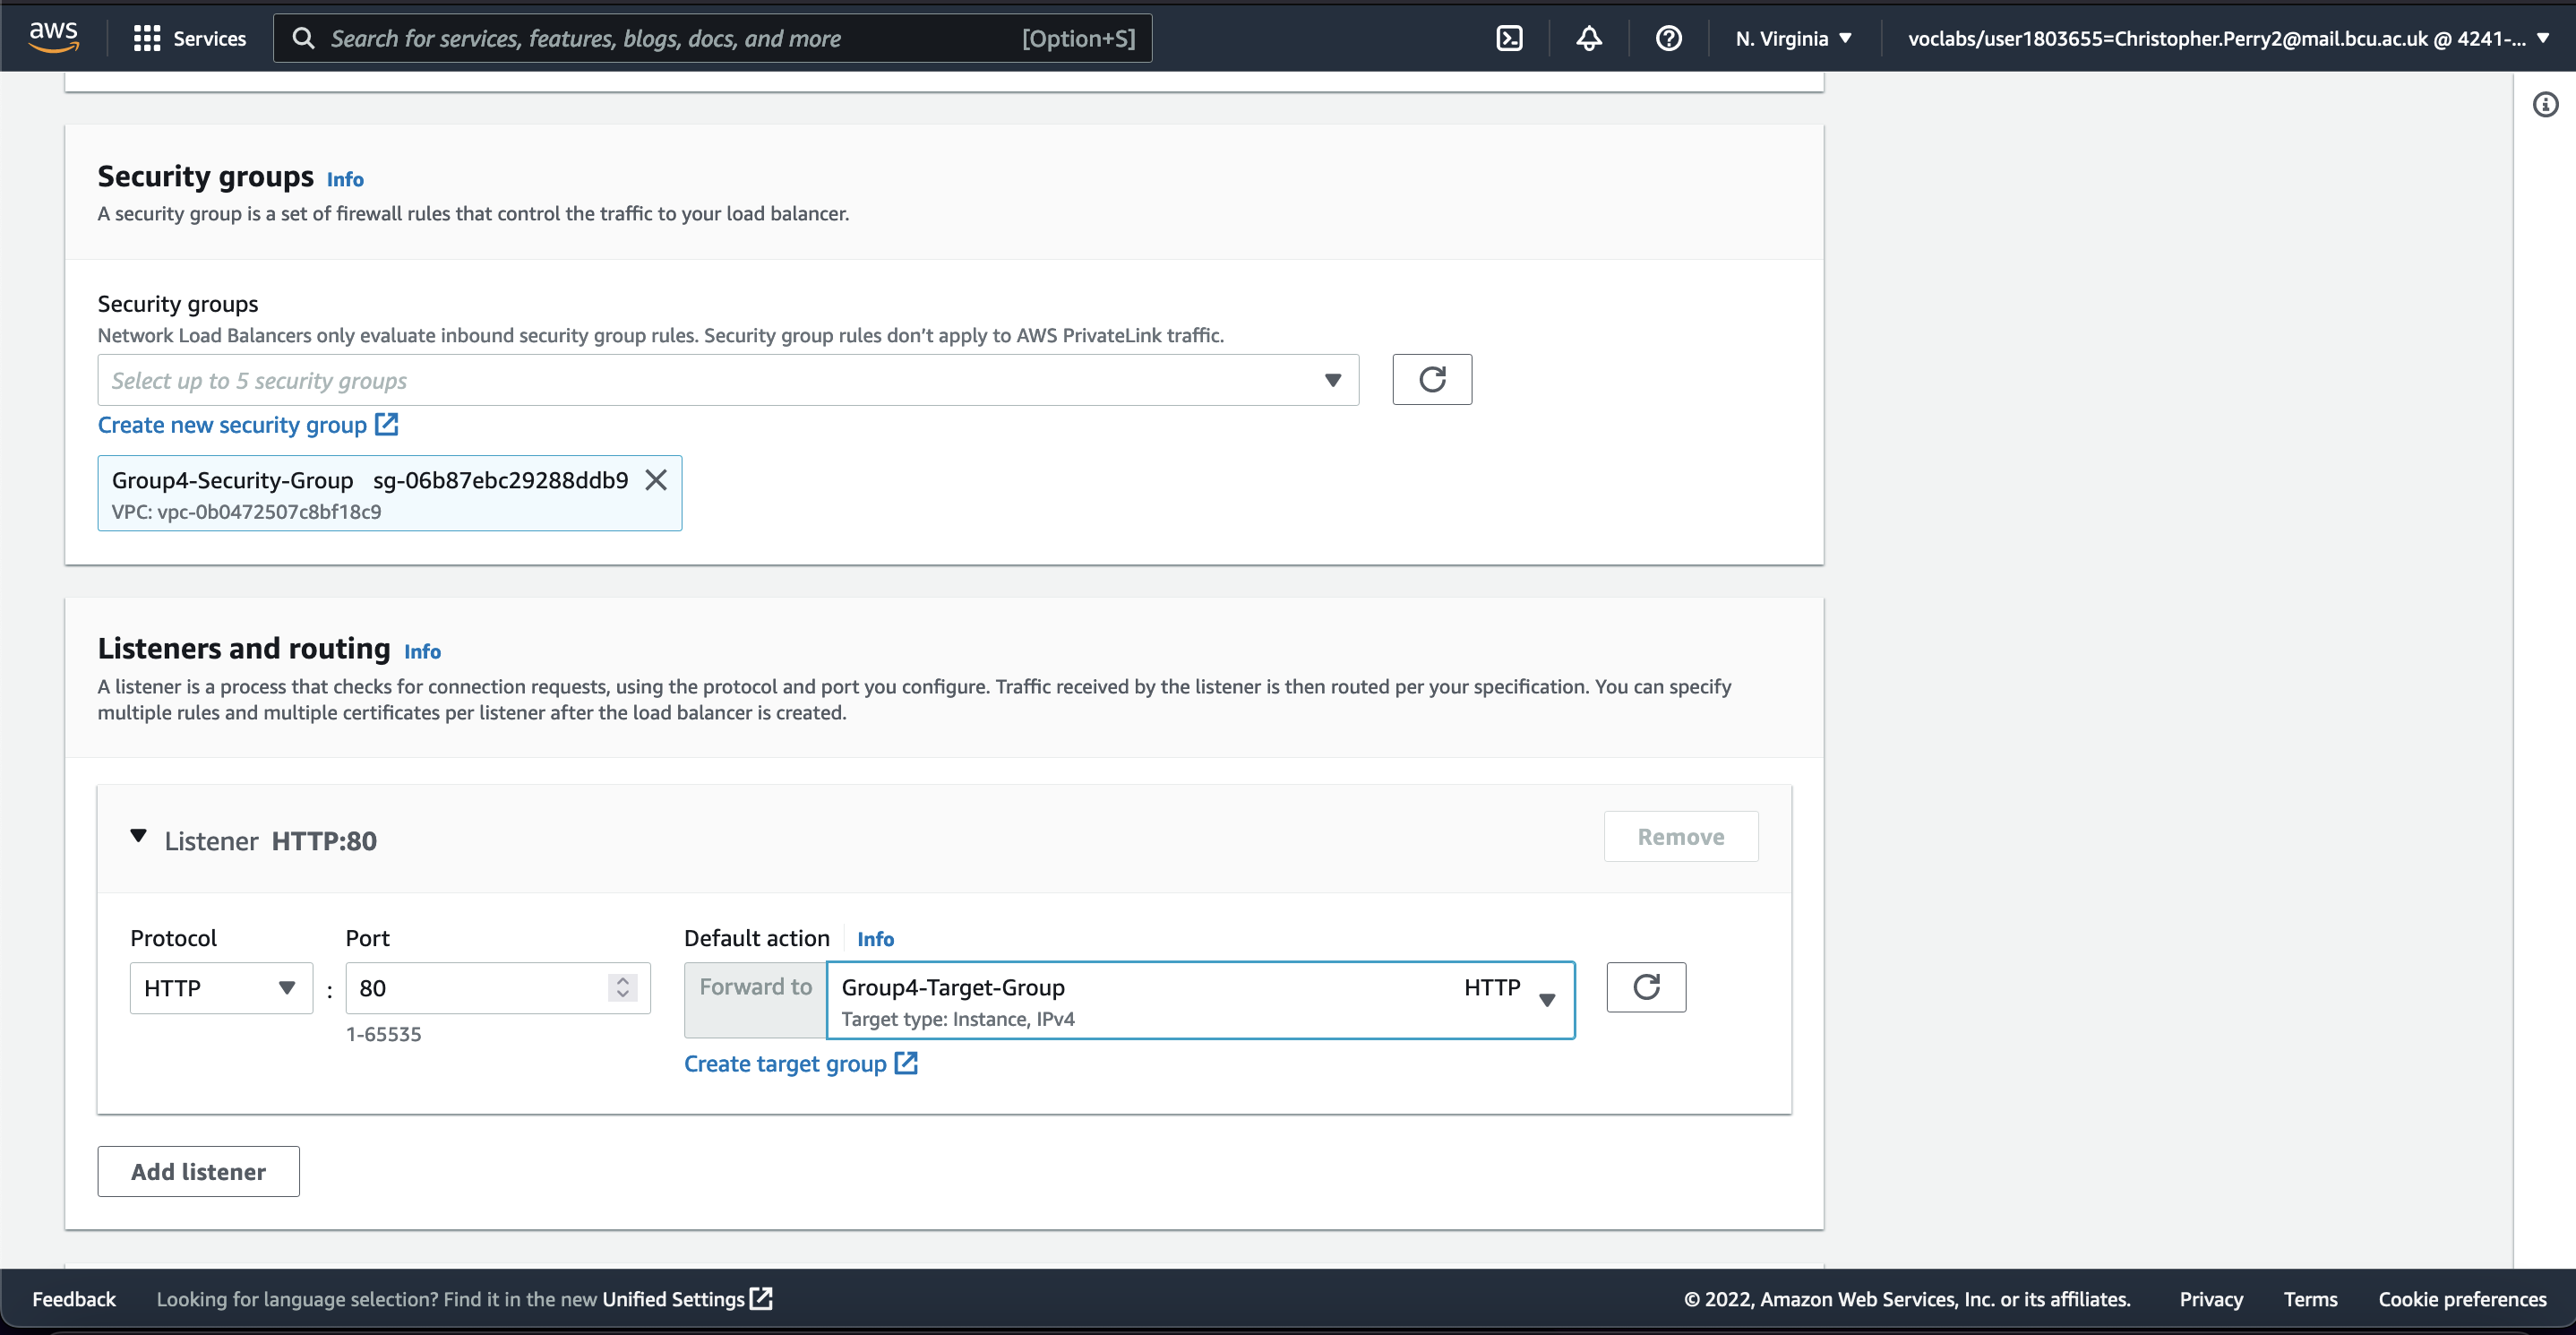
\includegraphics[width=120mm]{resources/elb/elb-security-groups-and-listeners}
	\caption{Listeners and routing configuration.}
	\label{fig:elb-security-groups}
\end{figure}

Unfortunately, a Global Accelerator could not be created due to permission issues with the access given to the accounts
used to develop this deployment.

\begin{figure}[!htbp]
	\centering
	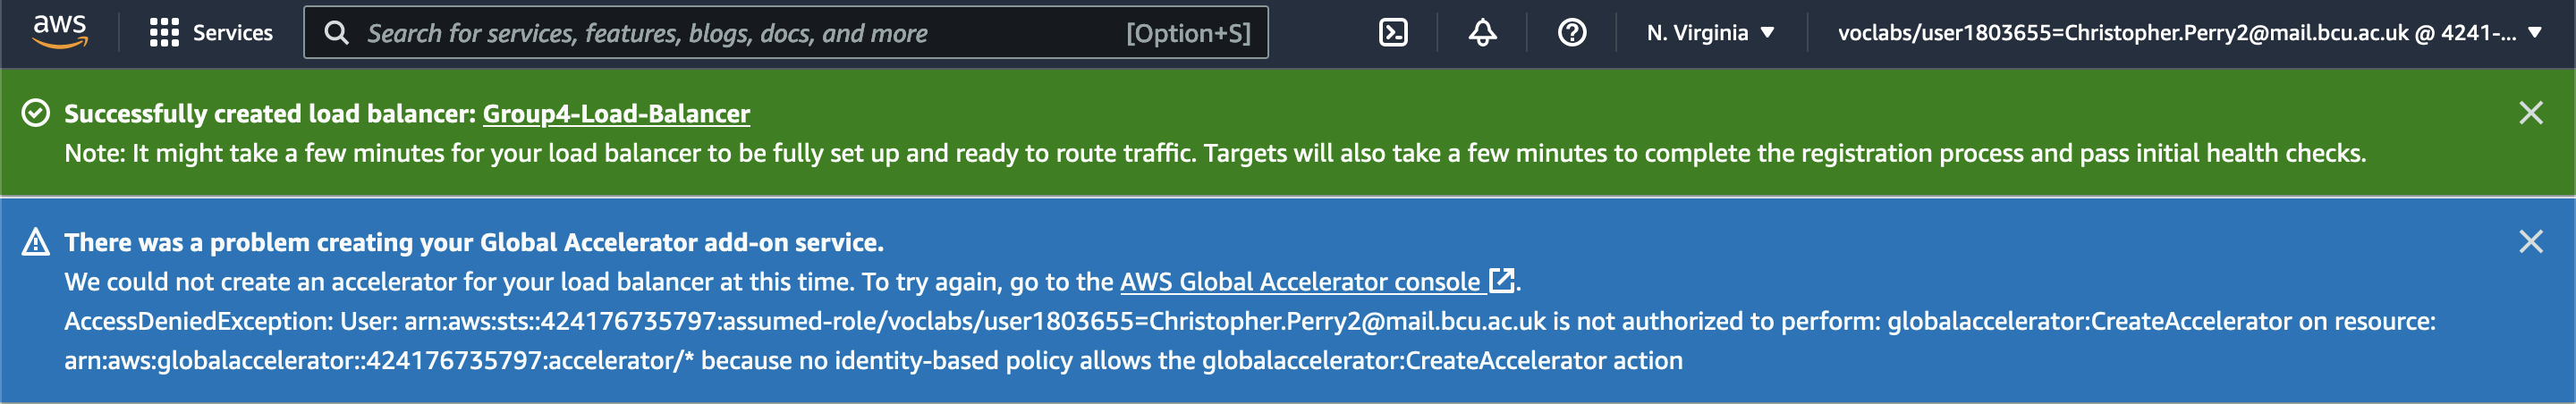
\includegraphics[width=120mm]{resources/elb/elb-accelerator}
	\caption{Unable to create a Global Accelerator.}
	\label{fig:elb-accelerators}
\end{figure}

\begin{figure}[!htbp]
	\centering
	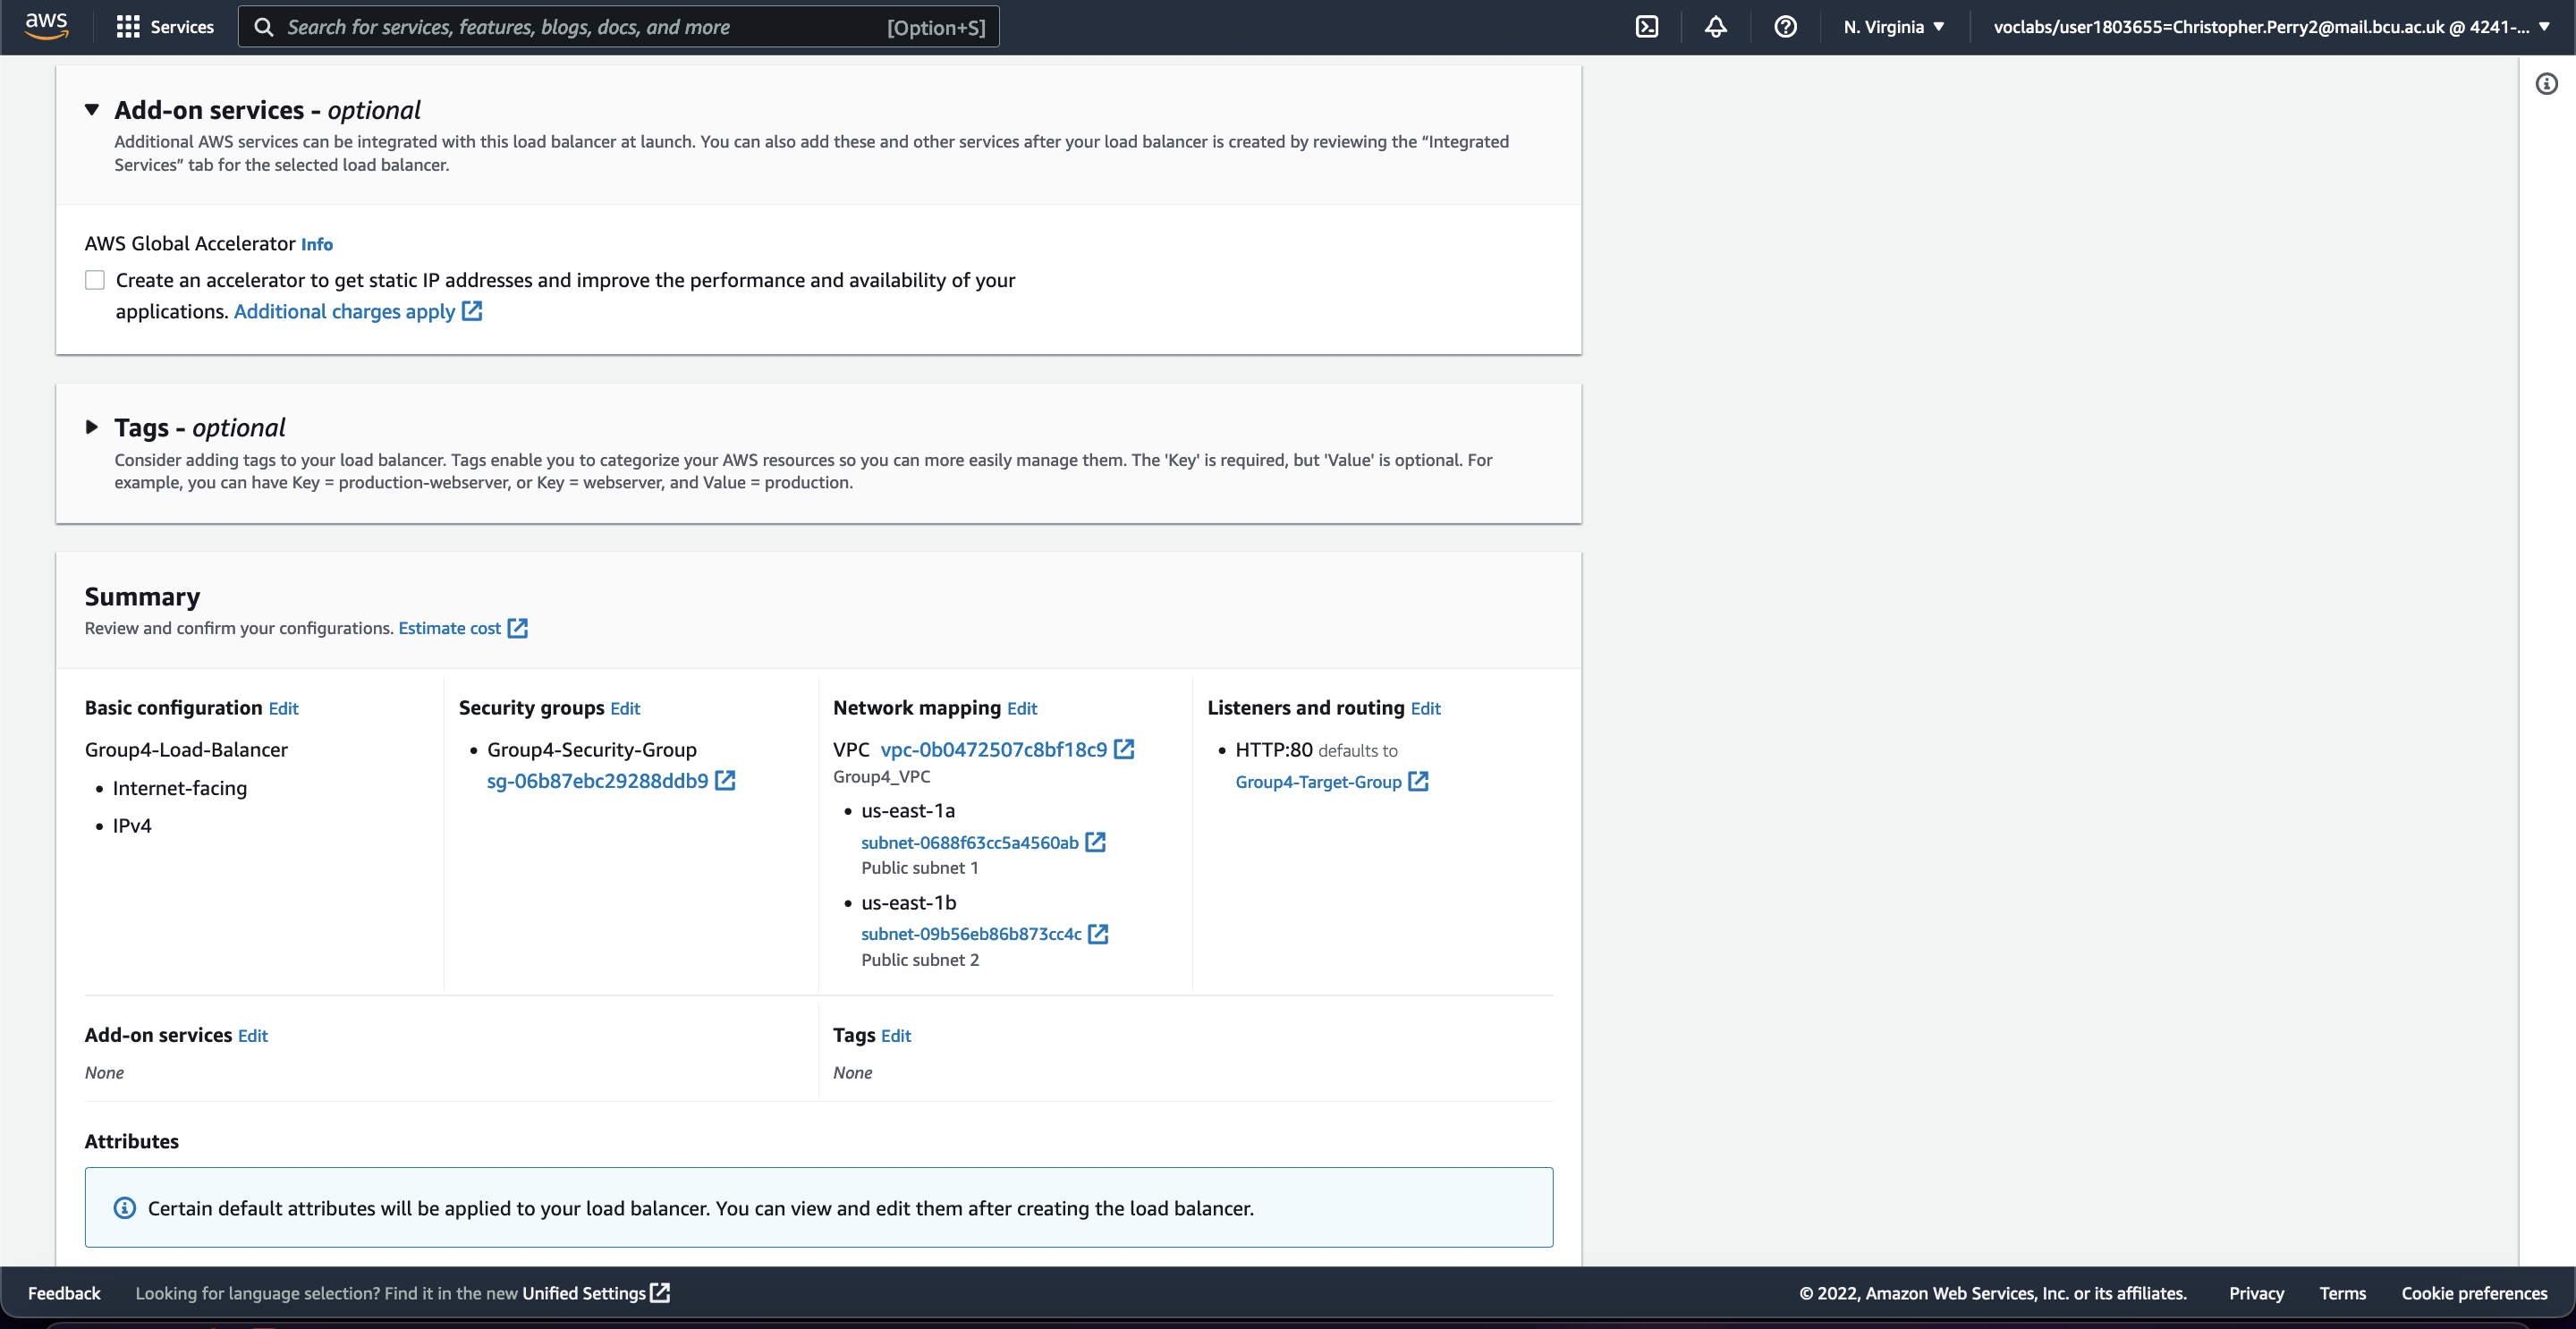
\includegraphics[width=120mm]{resources/elb/elb-summary}
	\caption{Final load balancer summary.}
	\label{fig:elb-summary}
\end{figure}

\clearpage
The load balancer has now been created.

\begin{figure}[!htbp]
	\centering
	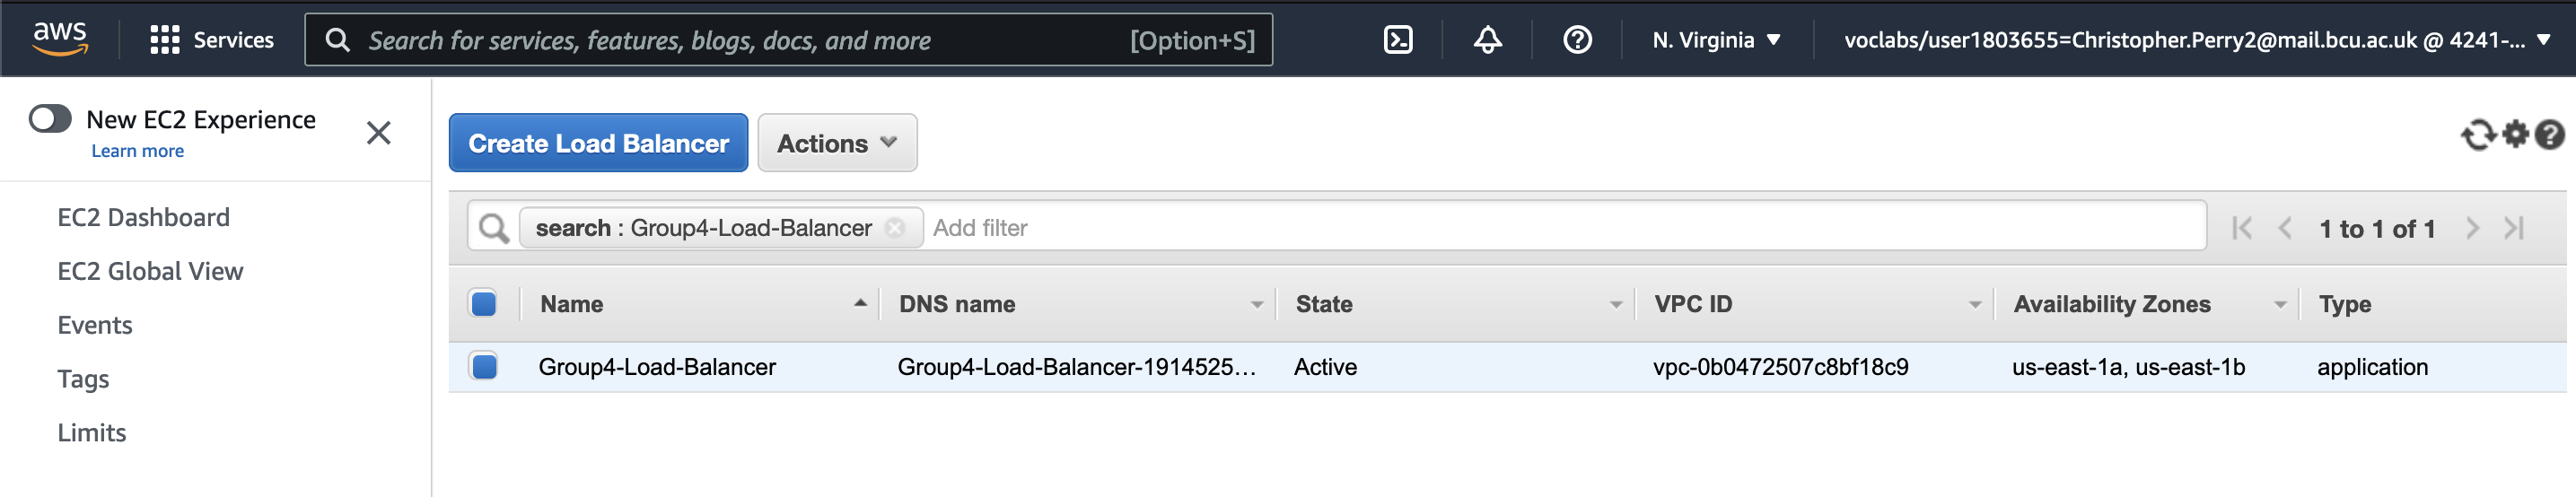
\includegraphics[width=\textwidth]{resources/elb/elb-created}
	\caption{Load balancer list view.}
	\label{fig:elb-created}
\end{figure}

When the load balancer is visited at
\href{http://http://group4-load-balancer-1914525647.us-east-1.elb.amazonaws.com/}{http://http://group4-load-balancer-1914525647.us-east-1.elb.amazonaws.com/},
the website is shown.

\begin{figure}[!htbp]
	\centering
	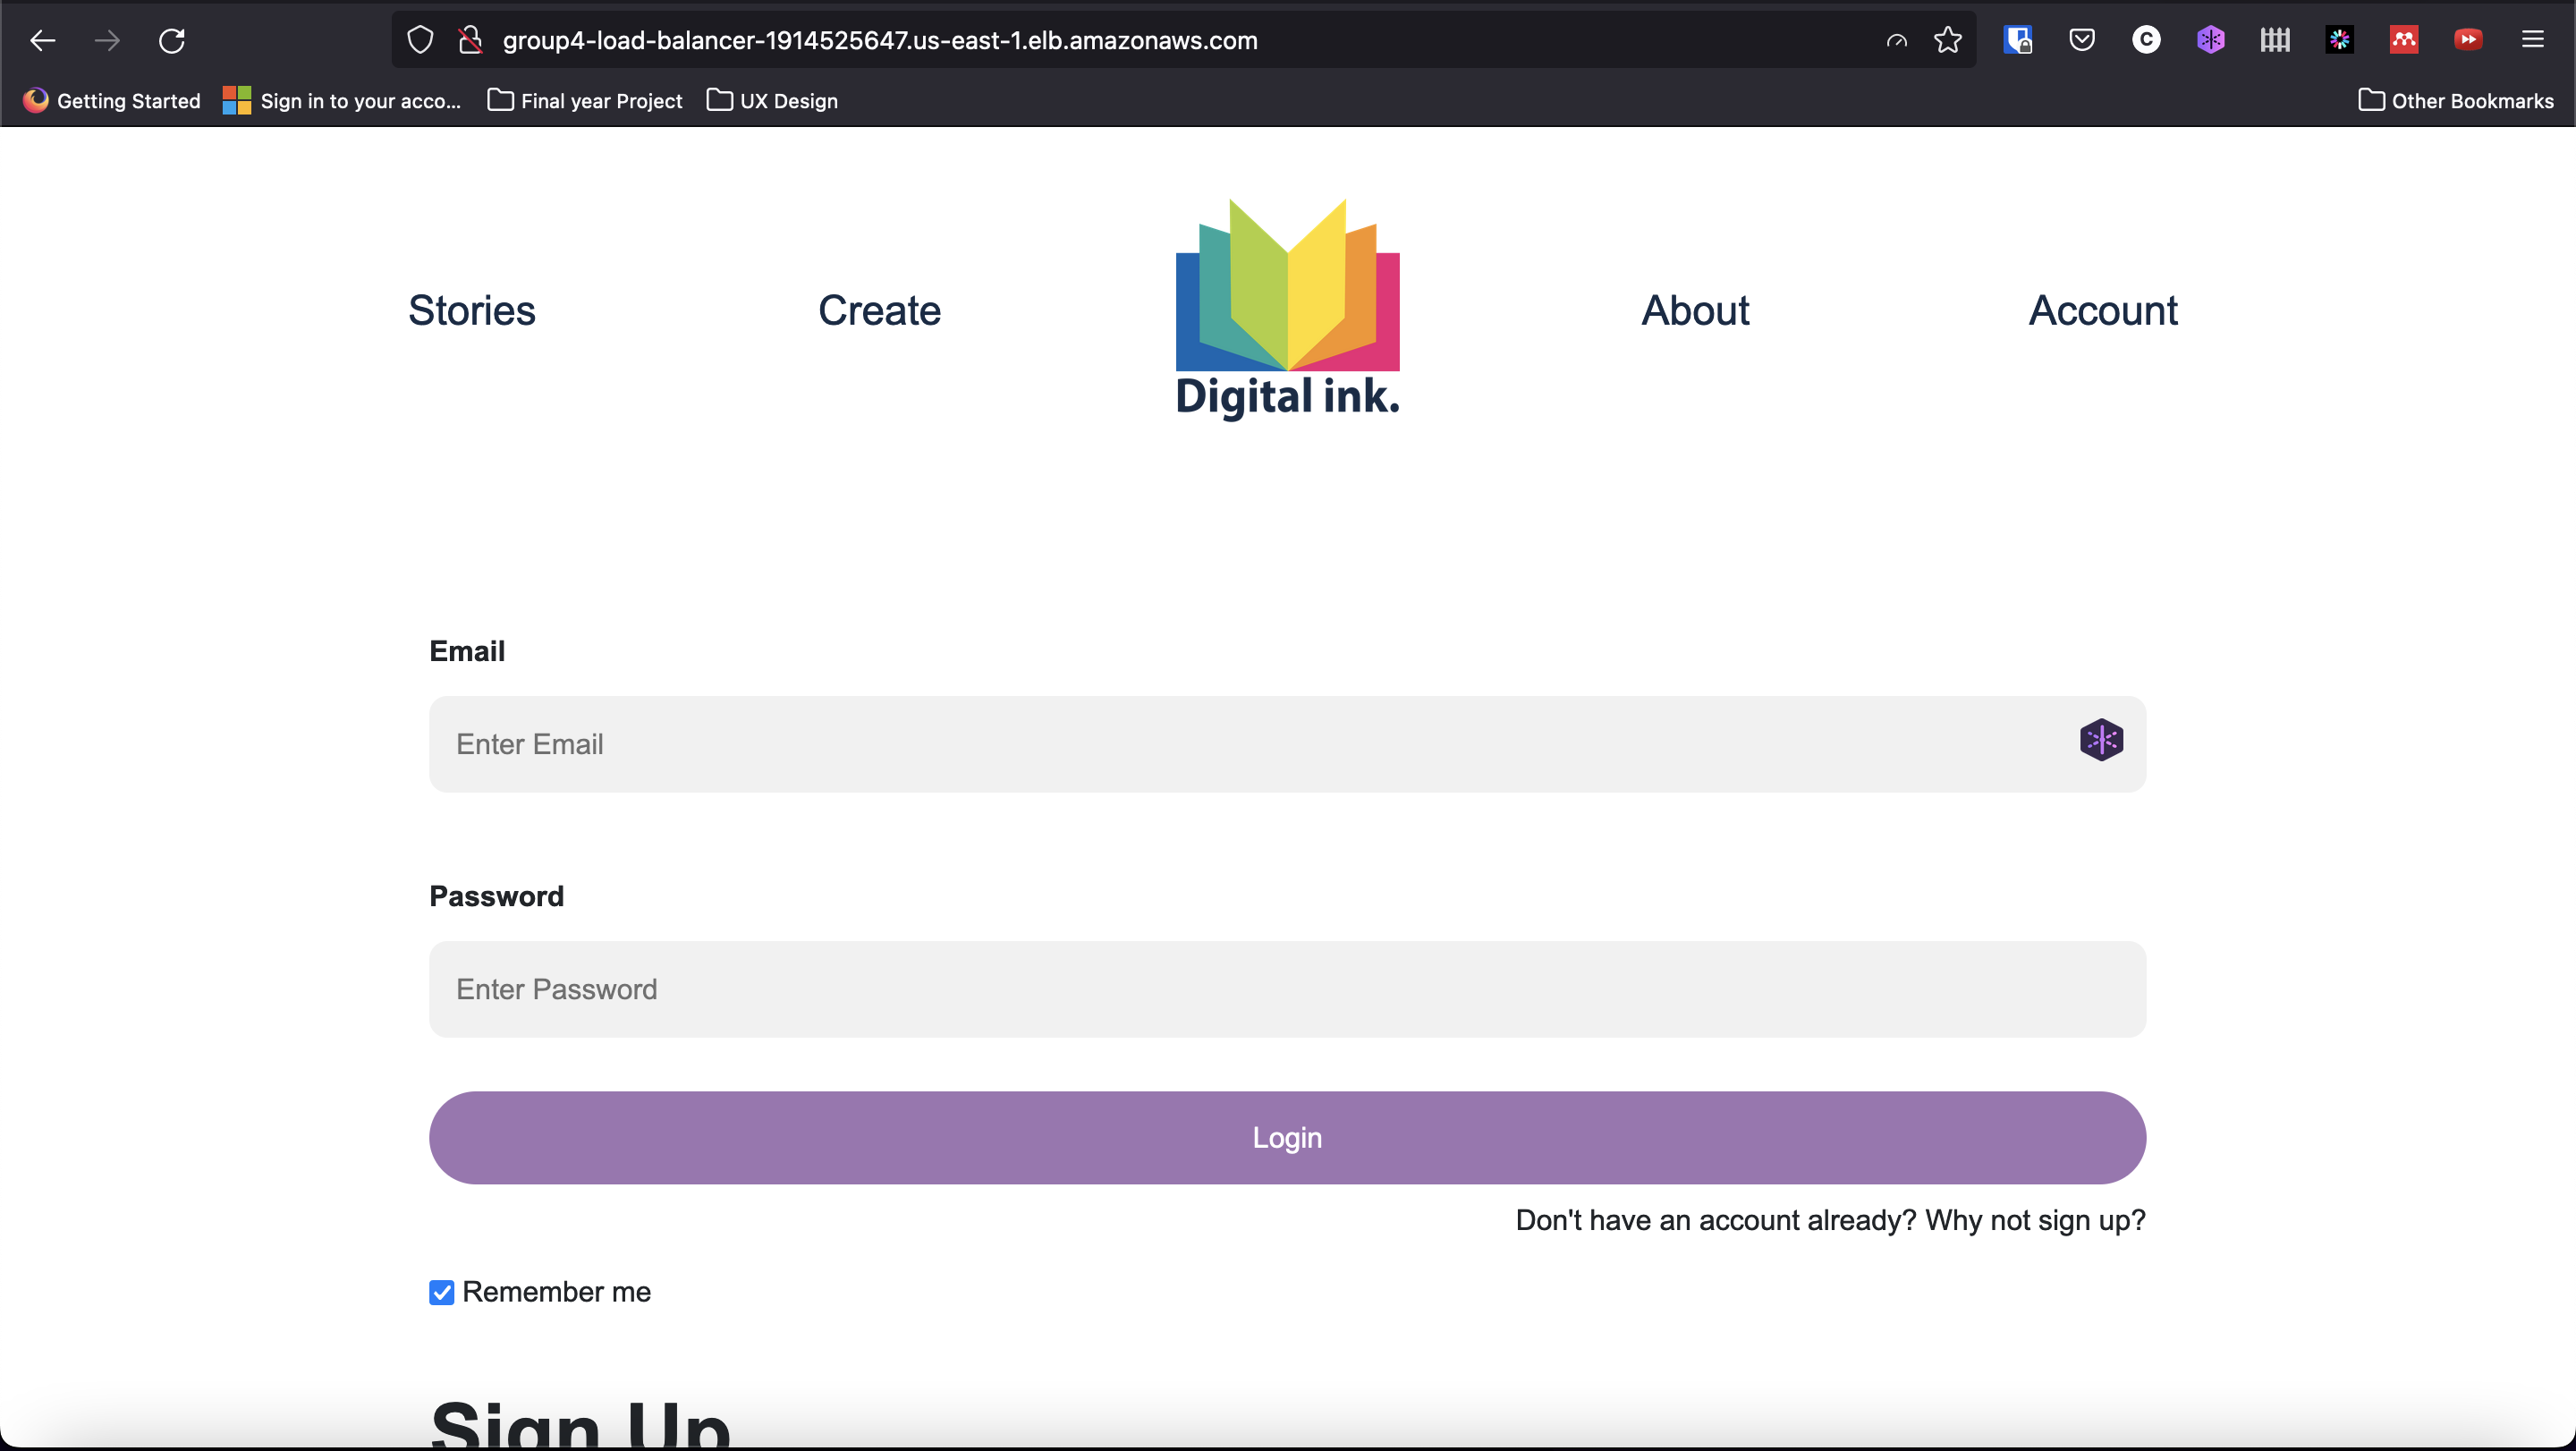
\includegraphics[width=\textwidth]{resources/elb/elb-working}
	\caption{Load balancer basic functionality test.}
	\label{fig:elb-working}
\end{figure}
